% !TEX root = LF-IMAPol.tex

\chapter{Notion of lexical function {\upshape [}LF\verythinspace{\upshape ]}}\label{chap:NotionLF}

This chapter presents the notion of lexical function -- hereafter, LF -- in nine steps:

\begin{itemize}

\item \nameref*{sec:LexMathFunctions} (\sectref{sec:LexMathFunctions})

\item \nameref*{sec:characStandardLFs} (\sectref{sec:characStandardLFs})

\item \nameref*{sec:LFParaSynt} (\sectref{sec:LFParaSynt})

\item \nameref*{sec:LFcombination} (\sectref{sec:LFcombination})

\item \nameref*{sec:PofS} (\sectref{sec:PofS})

\item \nameref*{sec:regularitiesInLFs} (\sectref{sec:regularitiesInLFs})

\item \nameref*{sec:descriptionTemplateLF} (\sectref{sec:descriptionTemplateLF})

\item \nameref*{sec:systemSimpleStandardLFs} (\sectref{sec:systemSimpleStandardLFs})

\item \nameref*{sec:descriptiveReliabilityOfLFs} (\sectref{sec:descriptiveReliabilityOfLFs})

\end{itemize}

\section{What is an LF?}\label{sec:LexMathFunctions}

\subsection{Definition of the notion of LF}\label{sec:LFDefinitionNotion}

A \notion{lexical function}\index[notion]{lexical function}\index[notion]{LF|see{lexical function}} is similar to a \emph{function} in the mathematical sense of the term. Recall that a \emph{mathematical}\index[notion]{lexical function!\tld\ vs mathematical function@\tld\ vs. mathematical function}\index[notion]{mathematical function} function $f$ is a relation\index[notion]{relation} between two sets $A$ and $B$ such that:

\begin{itemize}

\item $f$ applies to each individual element $a_i$ of $A$, called $f$'s \emph{argument} -- this application is denoted as $f(a_i)$;

\item $f(a_i)$ returns, in constant proportion, an element $b_i$ of $B$, called $f(a_i)$'s \emph{value}: $f(a_i) = b_i$;

\item by the application $f(a_i)$, each $a_i$ is associated to one and only one $b_i$.

\end{itemize}

For instance, arithmetical function $f_1$ specified by the formula $f_1(x) = x + 3$ is a relation that associates ($\mapsto$) to any positive integer $x$ another positive integer that is greater by three: $0 \mapsto 3$, $1 \mapsto 4$, $2 \mapsto 5$, ...

In the case of \emph{lexical} functions, the arguments and the values are, of course, not numbers:

\begin{itemize}

\item the \notion{argument} of an LF\index[notion]{argument of an LF}\index[notion]{lexical function!argument of a \tld} \lf{f} is a particular lexical unit L of the language under description;

\item \phantomsection\label{txt:valueOfAnLF}the \notion{value}\index[notion]{value of an LF|emph}\index[notion]{lexical function!value of a \tld|emph} of its application\index[notion]{application of an LF}\index[notion]{lexical function!application of a \tld} to L -- i.e., \lfappl{f}{L} -- is a set of (quasi-)synonymous lexical entities\index[notion]{lexical entity} that represent alternative choices for the expression of a given meaning.\footnote{The notions of lexical units and lexical entities have been defined in \chapref{chap:preliminaryNotions}, \sectref{sec:lexicalNotions}.}

\end{itemize}

The lexical entities that constitute the value of an LF application can be lexemes\index[notion]{lexeme}, idioms\index[notion]{idiom}, collocations\index[notion]{collocation}, compounding elements\index[notion]{compounding!\tld\ element} or derivational affixes\index[notion]{affix!derivational \tld}. The LF application \Next is an illustration with the LF \lf{A\tsub{1}}: adjective that typically characterizes the DSyntA~\syntDname{I} of its argument L (see \chapref{chap:paraLFs}, [\ref{lf:A-i}], p.\thinspace\pageref{lf:A-i}); in this case, L is \textsc{doubt}\tsub{(V)} and its DSyntA~\syntDname{I} the person who doubts.

\begingroup
\small

\ex. \begingroup\setlength{\tabcolsep}{2pt}
\begin{tabular}[t]{ l l p{7cm} }
\lfappl{A\tsub{1}}{\textit{doubt}\tsub{(V)}} & = & \textit{doubtful}\textbf{,} \textit{in doubt}\tsub{(N)} \\
\end{tabular}\label{ex:illustrationA1}\endgroup

\endgroup\index[lf]{Ai@\lf{A\tsub{i}}!\lf{A\tsub{1}}}

The equality \Last tells us that the LF \lf{A\tsub{1}} establishes a relation between the lexical unit \textsc{doubt}\tsub{(V)} and the set of near-synonymous lexical entities: the lexeme\index[notion]{lexeme} \textsc{doubtful} and the collocation\index[notion]{collocation} \textit{in doubt}.\footnote{The phrase \textit{in doubt} is a deep-syntactic adjective (on deep parts of speech, see \sectref{sec:notionPdD}, p.\thinspace\pageref{sec:notionPdD}).}

\begin{soundboxnotitle}

We use the term \notion{value} (of an LF) either to refer to a set of alternative lexical entities or, as a shortcut, to one of these lexical entities. For instance, we can say that the lexeme \textsc{doubtful} is a value of \lfappl{A\tsub{1}}{\textit{doubt}\tsub{(V)}}, where \textit{a value} is an abbreviation for \textit{an element of the value}. Similarly, we write formulas such as \mbox{``L\enskip{\small $\equiv$}\enskip\lfappl{Syn}{L}''} (cf. \sectref{sec:classeFLParadigmatiques}, p.\thinspace\pageref{txt:RSyn}) to state that the lexical unit L is equivalent to one of its synonyms (and not, of course, to the set of its synonyms).

\end{soundboxnotitle}

Let us now propose a definition of lexical functions.

\begin{notiondefinition}{lexical function}
A \notion{lexical function}\index[notion]{lexical function|emph} \lf{f} is a function such that \\*[2pt]
\setlength{\tabcolsep}{.5pt}\begin{tabular}{ p{0.2cm} >{\raggedright\arraybackslash}p{11cm} }
\SpecDiff & it expresses a particular meaning \sigmaF; \\
\SpecDiff & it applies to a lexical unit L as its argument -- this application
            being denoted as \lfappl{f}{L}; \\
\SpecDiff & it returns as value a set of (quasi-)synonymous lexical entities
            each of which expresses~\sigmaF\ as a function of L. \\
\end{tabular}
\end{notiondefinition}\index[notion]{argument of an LF}\index[notion]{lexical function!argument of a \tld}\index[notion]{application of an LF|emph}\index[notion]{lexical function!application of a \tld|emph}\index[notion]{lexical function!value of a \tld}\index[notion]{value of an LF}

This definition entails that LFs model such selection of lexical expressions\index[notion]{lexical selection} for a given meaning \sigmaF\ that is contingent upon the lexical expression of another meaning with which \sigmaF\ is combined. Let us explain this.

Linguistic meanings can belong to two major classes from the viewpoint of their lexical expression: to an open class of \emph{free} meanings or to a closed class of \emph{constrained} meanings.

\begin{soundbox}{Free vs. constrained meanings and lexical functions}
A \notion{free meaning}\index[notion]{meaning!free \tld|emph} is directly expressible by a lexical means with no regard for other lexical choices made in the production of the same sentence -- e.g., `not expected' can be freely expressed as \textit{unexpected}. No matter what exactly is not expected -- \textit{birth}, \textit{thunderstorm} or \textit{behavior}, it can be characterized as \textit{unexpected}. This is, so to speak, the default situation.

A \notion{constrained meaning}\index[notion]{meaning!constrained \tld|emph}\label{txt:constrainedMeaning}, by contrast, is lexically expressed depending on another lexical choice. Thus, the meaning `intense \lfgp{X}' has to be lexically expressed as a function of the lexical expression of `X': `intense desire' can be expressed as \textit{burning desire}, and `intense despair' can be expressed as \textit{deep despair} (while *\textit{deep desire} and *\textit{burning despair} are both ill-formed).

It is for constrained meanings that LFs come into play. Each LF \lf{f} is associated to a constrained meaning -- written \sigmaF: an application \lfappl{f}{L} computes the lexical expression of \sigmaF as a function of the lexical unit L.
\end{soundbox}

The expression ``meaning \sigmaF\ associated to an FL'' is an approximation. In fact, the semantic content \sigmaF\ is not necessarily a genuine meaning. Two cases can be distinguished.\footnote{\textcite{KahanePolguere2001-e} proposes a formal modeling of the meaning expressed by each LF, as well as of \emph{combinations} of LFs  presented in \sectref{sec:LFcombination} below.}

First, \sigmaF\ is a genuine meaning -- e.g., `the one who does [L]' for the LF \lf{S\tsub{1}} (\chapref{chap:paraLFs}, [\ref{lf:S-i}], p.\thinspace\pageref{lf:S-i}), as in \lfappl{S\tsub{1}}{\textit{build}} = \textit{builder}. Alternatively, the LF can correspond to a disjunction of genuine meanings -- e.g., \lf{Magn} (\chapref{chap:syntLFs}, [\ref{lf:Magn}], p.\thinspace\pageref{lf:Magn}) corresponds to `intense' (\textit{mad} [\textit{love}]), to `of big magnitude' (\textit{heavy} [\textit{weight}]), to `to a high degree' ([\textit{stubborn}] \idiom{\textit{as a mule}}), etc. Note that \sigmaF\ can be a zero meaning: cf. support verbs\index[notion]{support verb}\index[notion]{verb!support \tld}, such as \lf{Oper\tsub{i}}\index[lf]{Operi@\lf{Oper\tsub{i}}} (\chapref{chap:syntLFs}, [\ref{lf:Oper-i}], p.\thinspace\pageref{lf:Oper-i}).

Second, \sigmaF\ is, strictly speaking, not a meaning, but an indication of meaning identity of L and \lfappl{f}{L}:

\begin{itemize}

\item with preservation of L's part of speech; see, for instance, the LF \lf{Syn} (\chapref{chap:paraLFs}, [\ref{lf:Syn}], p.\thinspace\pageref{lf:Syn}): \lfappl{Syn}{\textit{buttocks}} = \textit{butt};

\item with change of the part of speech; see, for instance, the LF \lf{S\tsub{0}} (\chapref{chap:paraLFs}, [\ref{lf:S0}], p.\thinspace\pageref{lf:S0}): \lfappl{S\tsub{0}}{\textit{pursue}} = \textit{pursuit}.

\end{itemize}

To conclude this introductory presentation of the notion of LF, let us stress that the meaning \sigmaF\ of an LF \lf{f} determines its \notion{domain of application}\index[notion]{domain of application of an LF|emph}\index[notion]{application of an LF!domain of \tld|emph}\index[notion]{lexical function!domain of application of a \tld|emph}, i.e. the set of its possible arguments: the meanings of the latter must be compatible with \sigmaF. Thus, the above-mentioned LF \lf{A\tsub{1}} takes as arguments only lexical units with predicative meanings (\chapref{chap:preliminaryNotions}, \sectref{sec:semanticNotions}). As a rule, two situations can present themselves:

\begin{itemize}

\item application of an LF to a lexical unit that does not belong to its domain -- i.e., to an illegitimate argument\index[notion]{argument of an LF!illegitimate \tld}\index[notion]{lexical function!illegitimate argument of a \tld}; for instance: *\lfappl{A\tsub{1}}{\textit{poppy}}, since the noun \textsc{poppy} is not predicative\index[notion]{predicativity};

\item application of an LF to a legitimate argument that returns an empty value\index[notion]{lexical function!empty value of a \tld}\index[notion]{value of an LF!empty \tld}\footnote{More precisely, the value is the empty set \{\thinspace\}.} in the given language (no lexical entity); for instance, \lfappl{A\tsub{1}}{\textit{swim}\tsub{(V)}} returns an empty value, since there is no special adjective in English to characterize somebody who is swimming.\footnote{The expression \textit{swimming} is an inflectional form (present participle) of the verb \textsc{swim}\tsub{(V)}, whose use is accounted for by the grammar.}\index[notion]{grammar}

\end{itemize}

\paragraph*{LFs and lexical networks.}

A natural language lexicon\index[notion]{lexicon!structure of the \tld} is essentially a huge set of lexical entities\index[notion]{lexical entity} connected by a set of relations: in other words, it is a \notion{lexical network}\index[notion]{lexical network}\index[notion]{network \lfgp{see also \textit{graph}}!lexical \tld}. LFs participate in the structuring of the lexicon in a fundamental way: each LF application \lfappl{f}{L} is equivalent to an elementary subnetwork. This is illustrated in \figref{fig:LFEquivLN-PROMISE} with two LF applications involving the lexeme \textsc{promise}\tsub{(N)} as argument.

\begin{figure}

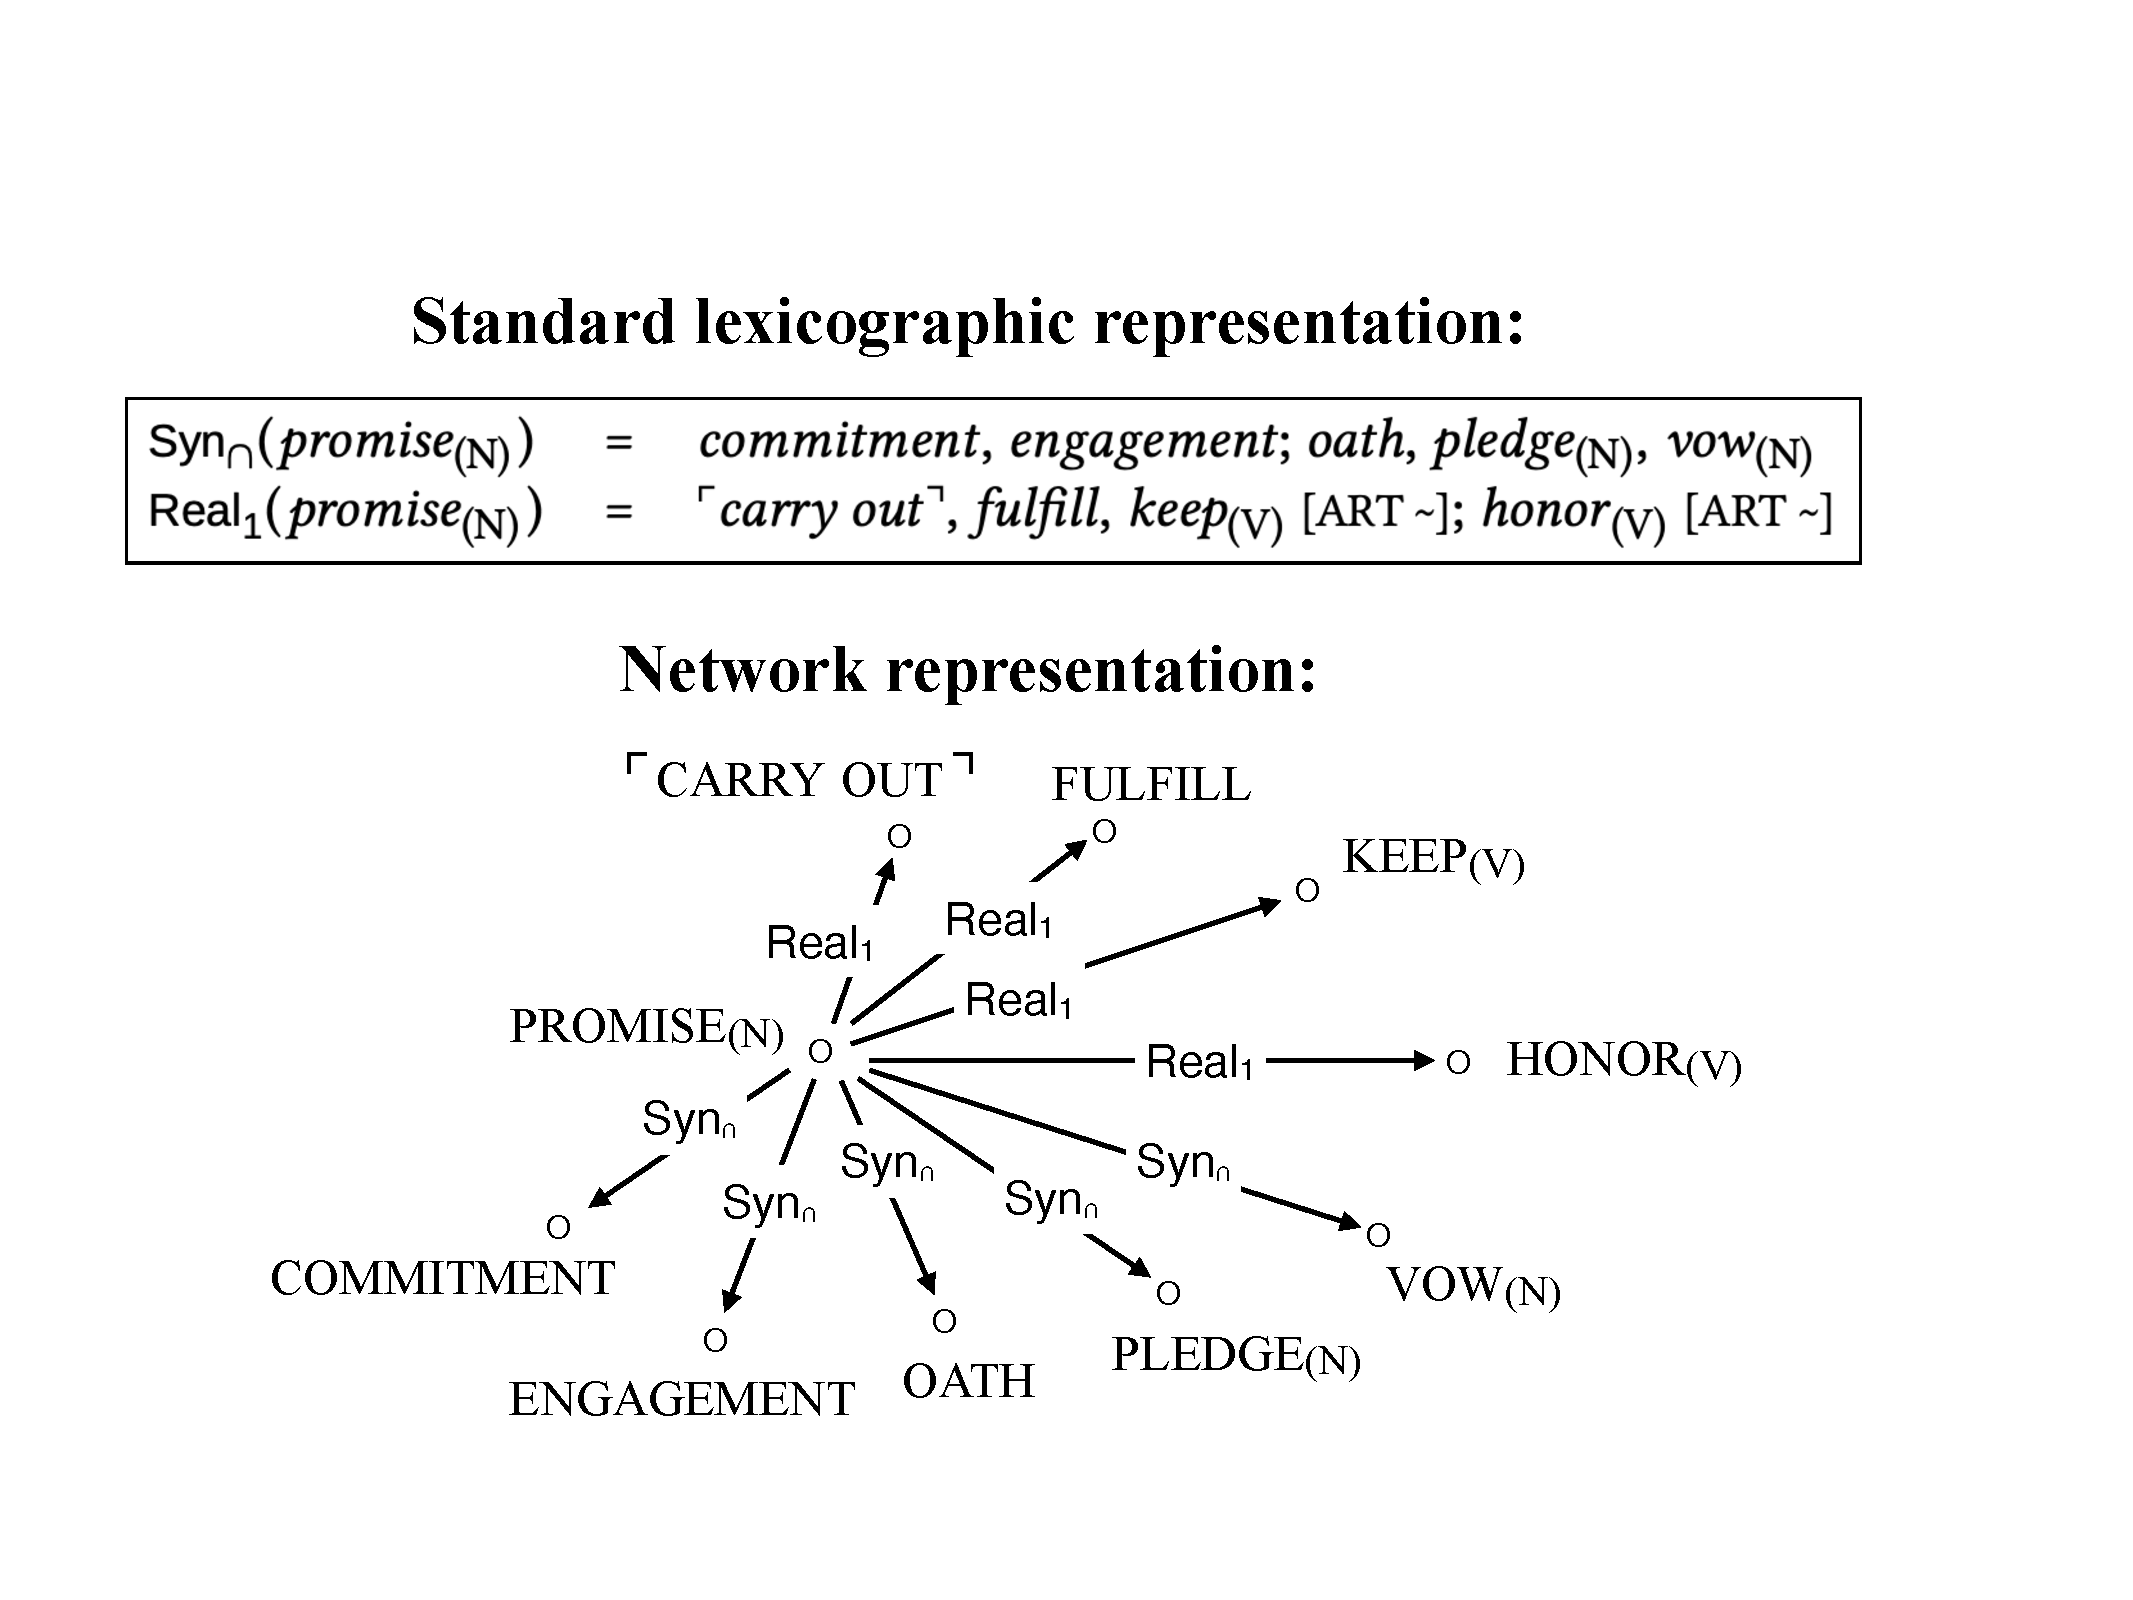
\includegraphics[width=9.5cm]{Fig/NotionLF/LFEquivLN-PROMISE.pdf}
\caption{Lexical network representing a set of LF applications}\label{fig:LFEquivLN-PROMISE}
\end{figure}\index[lf]{Syn@\lf{Syn}!\lf{Syn\tsub{$\cap$}}}\index[lf]{Reali@\lf{Real\tsub{i}}!\lf{Real\tsub{1}}}

%\begin{longtable*}[l]{ l l p{8cm} }
%\lfappl{Syn\tsub{$\cap$}}{\textit{promise}\tsub{(N)}} & = & \textit{commitment}\textbf{,} \textit{engagement}\textbf{;} \textit{oath}\textbf{,} \textit{pledge}\tsub{(N)}\textbf{,} \textit{vow}\tsub{(N)} \\
%\lfappl{Real\tsub{1}}{\textit{promise}\tsub{(N)}} & = & \idiom{\textit{carry out}}\textbf{,} \textit{fulfill}\textbf{,} \textit{keep}\tsub{(V)} \lfgp{\textsc{art} \tld}\textbf{;} \textit{honor}\tsub{(V)} \lfgp{\textsc{art} \tld} \\
%\end{longtable*}

The important issue of the structuring of lexical networks by LFs is considered in \chapref{chap:lexicalNetwork}.

\subsection{Notation for LF applications}\label{sec:notationForLFApplications}

Throughout this book, we use a set of notations\index[notion]{notation for LF application}\index[notion]{application of an LF}\index[notion]{lexical function!application of a \tld} (writing conventions and symbols) to present examples of LF applications. The general format of presentation for an LF application is as follows:

\begingroup
\small

\ex. \begingroup\setlength{\tabcolsep}{2pt}
\begin{tabular}[t]{ l l p{7cm} }
\lfappl{S\tsub{0}}{\textit{leave}\tsub{(V)}} & = & \textit{departure} \\
\end{tabular}\endgroup

\endgroup

The argument and the elements of the value of the LF are written in italics in the above formula -- though, technically, they are lexemes and should be written using the standard convention for lexical units: \textsc{leave}\tsub{(V)} and \textsc{departure}. However, this violation of conventions allows for easier legibility; additionally, values might not be lexical units (e.g., they can be collocations) and it is easier to use a uniform presentation for values, disregarding their lexical status. Note that lists of values in our examples are not necessarily complete; we often limit ourselves to only one value element.

As illustrated in example \Next, three symbols are used to separate the elements of an LF value: ``\textbf{,}'' for no or minimal semantic difference, ``\textbf{<}'' for the difference of degree, and ``\textbf{;}'' for a significant semantic difference.

\begingroup
\small

\ex. \begingroup\setlength{\tabcolsep}{2pt}
\begin{tabular}[t]{ l l >{\raggedright\arraybackslash}p{8cm} }
\lfappl{Magn}{\textit{salary}} & = & \textit{big}\textbf{,} \textit{generous}\textbf{,} \textit{hefty}\textbf{,} \textit{large}\textbf{,} \textit{substantial} \textbf{<} \textit{enormous}\textbf{,} \textit{huge}\textbf{,} \textit{massive}\textbf{;} \textit{exorbitant} \\*
\multicolumn{3}{>{\raggedright\arraybackslash}p{10cm}}{{\footnotesize [The value \textit{exorbitant} expresses an additional semanteme:  `too much'.]}} \\
\end{tabular}\endgroup

\endgroup

The ``\fused'' symbol used in \Next below indicates a fused\index[notion]{fusion}\index[notion]{value of an LF!fused \tld}\index[notion]{lexical function!fused value of a \tld} value element (see \sectref{sec:quidProQuoValues}, p.\thinspace\pageref{par:fusedValuesSyntLFs}).

\begingroup
\small

\ex. \begingroup\setlength{\tabcolsep}{2pt}
\begin{tabular}[t]{ l l >{\raggedright\arraybackslash}p{8cm} }
\lfappl{Magn}{\textit{amaze}} & = & \textit{utterly}\textbf{,} \fused\textit{stun}\tsub{(V)} {\footnotesize [$\equiv$ \textit{utterly amaze}]} \\
\end{tabular}\endgroup

\endgroup

Finally, two indications can follow a given value element L′.

\begin{enumerate}

\item \label{par:valueGP}The government pattern\index[notion]{government pattern!\tld\ of an LF value element|emph}\index[notion]{value of an LF!government pattern of an element of the \tld|emph}\footnote{On government patterns, see \chapref{chap:preliminaryNotions}, \sectref{sec:syntacticNotions}, p.\thinspace\pageref{txt:governmentPattern}.} of L′, written between square brackets, specifies the syntactic configuration that L′ can govern. This configuration is presented in simplified linear form; for instance in \Next below, where ``\tld'' stands for the LF's argument (\textit{kiss}\tsub{(N)}) and ``\textsc{art}'' stands for a determiner:

\begingroup
\small

\ex. \begingroup\setlength{\tabcolsep}{2pt}
\begin{tabular}[t]{ l l >{\raggedright\arraybackslash}p{8cm} }
\lfappl{Oper\tsub{1}}{\textit{kiss}\tsub{(N)}} & = & \textit{give} \lfgp{\textsc{art} \tld\ \textit{to} N\tsub{Y}} \\
\end{tabular}\endgroup

\endgroup

\item Semantic or grammatical constraints associated with L′ are introduced by a vertical bar ``\thinspace\constrbar\thinspace''; for instance:

\begingroup
\small

\ex. \begingroup\setlength{\tabcolsep}{2pt}
\begin{tabular}[t]{ l l >{\raggedright\arraybackslash}p{8cm} }
\lfappl{Oper\tsub{1}}{\textit{visit}\tsub{(N)}} & = & \textit{pay} \lfgp{\textsc{art} \tld\ \textit{to} N\tsub{Y}} \lfconstr{N\tsub{Y} denotes a person} \\
\end{tabular}\endgroup

\endgroup

\end{enumerate}

\section{Simple standard LFs}\label{sec:characStandardLFs}

The LFs as defined in \sectref{sec:LexMathFunctions} constitute a system\index[notion]{lexical function!system of standard \tlds}\index[notion]{system of standard LFs} built around a core of about seventy LFs, called \notion{simple standard LFs}\index[notion]{lexical function!standard \tld|emph}; they are referred to just as \textit{LFs} in the subsequent discussion. Let us present the fundamental properties of these LFs.

The set of LFs has been empirically identified over the last 60 years in the context of the study of typologically varied languages (first publication on LFs: \cite{ZolkovskijMelcuk1965-e}). The work on Russian and French Explanatory Combinatorial Dictionaries\index[notion]{dictionary!Explanatory Combinatorial \tld}\index[notion]{Explanatory Combinatorial!\tld\ Dictionary}\index[notion]{lexicography} has allowed the researchers to sharpen the LF system and to consolidate the very notion of LF, under the elaboration of lexical entries\index[notion]{lexical entry}, where LFs are systematically used \parencite{MelcukZholkovsky1984,MelcukZolkovskij2016,MelcukEtAl1984,MelcukEtAl1988,MelcukEtAl1992,MelcukEtAl1999,MelcukPolguere2007-e}. At the same time, Meaning-Text\index[notion]{Meaning-Text!\tld\ approach} research on \notion{syntactic paraphrasing}\index[notion]{paraphrase!syntactic \tld} \parencites{Milicevic2007}[Ch.~9]{Melcuk2013c-e} and dependency syntax\index[notion]{syntax!dependency \tld}\index[notion]{dependency!\tld\ syntax} \parencite{MelcukPertsov1987,Melcuk1988a,Melcuk2009a,Melcuk2015c,Melcuk2016b,Melcuk2021a} have heavily contributed to the maturation of the notion.

Three topics are discussed below: fundamental properties of LFs (\sectref{sec:FLStandard2Carac}), non-standard LFs (\sectref{par:nonStandardLFs}) and LFs in deep syntax (\sectref{sec:DSyntAndLFs}).

\subsection{Properties of simple standard LFs}\label{sec:FLStandard2Carac}

Simple standard LFs have two fundamental properties: a vast domain of application (\sectref{sec:vastDomainOfApplication}) and a vast range of possible values\index[notion]{value of an LF}\index[notion]{lexical function!value of a \tld} (\sectref{sec:vastRangeOfValues}). These properties follow from the character of the constrained meanings\index[notion]{meaning!constrained \tld} \sigmaF\ that simple standard LFs express.\footnote{On constrained meanings, see \sectref{sec:LFDefinitionNotion}, p.\thinspace\pageref{txt:constrainedMeaning}.}

The first property implies two other more specific properties: potential morphological expression of \sigmaF\ in natural languages (\sectref{sec:morphologicalExpressionSigmaF}) and universality of simple standard LFs (\sectref{sec:universality}).

\subsubsection{Vast domain of application}\label{sec:vastDomainOfApplication}

A given LF \lf{f} takes, in a given natural language, a large number of arguments: it has a vast domain of application\index[notion]{domain of application of an LF}\index[notion]{application of an LF!domain of \tld}\index[notion]{lexical function!domain of application of a \tld}. To put it differently, the meaning \sigmaF\ must be sufficiently vague (i.e., impoverished) to be compatible with a large set of lexical meanings to which it is supposed to be united\slashs{}associated.

Consequently, an \lf{f} involves a significant subset of a language's lexicon, and this subset is semantically rather heterogenous. Thus, for instance, one may wish to postulate a simple standard LF with meaning `young of L' to describe the following \notion{lexical relations}\index[notion]{lexical relation|emph}\index[notion]{relation!lexical \tld|emph}\phantomsection\label{txt:lexicalRelationIntro}:

\begingroup
\small

\ex. \begingroup\setlength{\tabcolsep}{2pt}
\begin{tabular}[t]{ l l l }
\textit{cat} & \lexRel{\lf{young of}} & \textit{kitten} \\
\textit{dog} & \lexRel{\lf{young of}} & \textit{puppy} \\*
\textit{pig} & \lexRel{\lf{young of}} & \textit{piglet} \\
\end{tabular}\endgroup\label{tab:youngOf}

\endgroup

This, however, would not be correct since this LF's meaning specifies a very constrained \notion{semantic class}\index[notion]{semantic!\tld\ class} of potential arguments: that of animate beings. Such a lexical relation can be described by an LF, but by a \emph{non-standard} LF\index[notion]{lexical function!non-standard \tld} (see \sectref{par:nonStandardLFs}, p.\thinspace\pageref{par:nonStandardLFs}).

\begin{soundboxnotitle}

A lexical relation \lf{LexRel} -- of any type -- between lexical units L and L′ is denoted as L\thinspace\lexRel{\lf{LexRel}}\thinspace L′.

\end{soundboxnotitle}

\subsubsection{Vast range of possible values}\label{sec:vastRangeOfValues}

The application \lfappl{f}{L} returns a large number of different values for different arguments: \lf{f} is, therefore, not a trivial relation. An LF that would express the meaning `of white color' would have a trivial value: \textsc{white}\tsub{(Adj)} for any lexical unit L. Such trivial cases must not be considered when identifying standard LFs.

\subsubsection{Potential morphological expression of \sigmaF}\label{sec:morphologicalExpressionSigmaF}

The first above property (vast domain of application) entails another significant property of standard LFs. Given their frequency in the language and their semantic regularity, one can expect the expression of \sigmaF\ by morphological means\index[notion]{morphology!morphological means}. This can happen, in a given language, either massively or sporadically; for instance:

\begin{itemize}

\item to implement the LF \lf{S\tsub{1}} (\chapref{chap:paraLFs}, [\ref{lf:S-i}], p.\thinspace\pageref{lf:S-i}), English uses the very productive derivational suffix\index[notion]{suffix!derivational \tld} \textsc{-er} (\textit{driv}+\textit{er}, \textit{advis}+\textit{er}, ...);

\item by contrast, one finds in French the unproductive nominal derivational suffix \mbox{\textsc{-aillon}} that expresses the complex LF \lf{AntiBon}\index[lf]{AntiBon@\lf{AntiBon}}\index[lf]{Bon@\lf{Bon}!AntiBon@\lf{AntiBon}} (\chapref{chap:syntLFs}, [\ref{lf:Bon}], p.\thinspace\pageref{lf:Bon}): {\smaller French}~\textit{avoc}+\textit{aillon} `bad lawyer' (from \textit{avocat} `lawyer'), \textit{écriv}+\textit{aillon} `bad writer' (from \textit{écrivain} `writer'), and a few other nouns.

\end{itemize}

\subsubsection{Universality of simple standard LFs}\label{sec:universality}

LFs that have the above properties are linguistically \notion{universal}\index[notion]{language-universal}; by this, we mean two things.

Firstly, each LF is supposed to be found in all or most world languages. We say \textit{most} because an LF can be trivial in a given language: it is always expressed there by the same linguistic means -- a given lexical unit or a given affix\index[notion]{affix}.

Secondly, the system of LFs proposed in the present volume is presumed complete. It is believed (until proven wrong) that one cannot find in a language a lexical relation with the above properties of simple standard lexical functions that would not be included in the proposed system.

Given\phantomsection\label{txt:LFNames} LFs' linguistic universality, it seems natural that their names\index[notion]{lexical function!\tld\ name} come from Latin, so that they are not linked to any specific contemporary language.\footnote{The LF \lf{Equip} (\chapref{chap:paraLFs}, [\ref{lf:Equip}], p.\thinspace\pageref{lf:Equip}), from {\smaller French}~\textit{équipage} `crew', is an exception.} To keep LF formulas relatively short, Latin sources are truncated to a maximum of four or five characters -- e.g., \lf{Syn}\index[lf]{Syn@\lf{Syn}}, from {\smaller Latin}~\textit{synonymum}. In a few cases, pseudo-Latin terms are used, preceded by an asterisk -- e.g., \lf{Conv\tsub{ijk}}\index[lf]{Convijk@\lf{Conv\tsub{ijk}}}, from {\smaller Latin}~*\textit{conversivum}.

\subsection{Non-standard LFs}\label{par:nonStandardLFs}\index[notion]{lexical function!non-standard \tld|emph}

Any natural language possesses an open set of constrained meanings\index[notion]{meaning!constrained \tld} \sigmaF\ such that:

\begin{itemize}

\item Each one of them is much richer than meanings of standard LFs.

\item Because of this, a \sigmaF\ can apply only to a semantically limited set of arguments; in point of fact, its domain of application\index[notion]{domain of application of an LF}\index[notion]{application of an LF!domain of \tld}\index[notion]{lexical function!domain of application of a \tld} is a clearly identifiable semantic field\index[notion]{semantic!\tld\ field} or a handful of lexical units. Quite frequently, its domain is even reduced to one lexical unit.

\item There is not much variability in its expression -- most of the time, just one lexical unit.

\end{itemize}

Such meanings are still expressed as a function of their argument and therefore they can be described by LFs, but by LFs of a completely different nature than standard LFs: these are \notion{non-standard LFs}.

Three examples are given in \Next: \lf{young of}, mentioned earlier in \ref{tab:youngOf}, which only applies to the semantic class\index[notion]{semantic!\tld\ class} of lexical units denoting higher-order animals; \lf{overprotective of their children}, which applies only to \textsc{parent}\tsub{(N)}, \textsc{mother}\tsub{(N)} and \textsc{father}\tsub{(N)} (and a few of their synonyms); \lf{of 366 days}, which applies only to the lexical unit \textsc{year}.

\begingroup
\small

\ex. \begingroup\setlength{\tabcolsep}{2pt}
\begin{tabular}[t]{ l l >{\raggedright\arraybackslash}p{6cm} }
\lfappl{young of}{\textit{cat}\tsub{(N)}} & = & \textit{kitten}\tsub{(N)} \\*
\lfappl{overprotective of her child}{\textit{mother}\tsub{(N)}} & = & \textit{helicopter}\tsub{(N)} \lfgp{\tld}  \\*
\lfappl{of 366 days}{\textit{year}} & = & \textit{leap}\tsub{(N)} \lfgp{\tld}  \\
\end{tabular}\endgroup

\endgroup

Non-standard LFs differ from standard LFs in the following aspects:

\begin{itemize}

\item They are not universal\index[notion]{language-universal}, but language-specific.

\item Their number in a given language is unlimited, and they cannot be theoretically foreseen.

\item They are so diverse that it is difficult to normalize them, and they have to be specified by the lexicographic definition\index[notion]{definition!lexicographic \tld} of their value.

\item Prototypically, they are not deep lexical units\index[notion]{lexical unit!deep \tld}: they do not appear in deep-syntactic structures\index[notion]{deep-syntactic!\tld\ structure [DSyntS]}\index[notion]{structure!deep-syntactic \tld\ [DSyntS]} and do not participate in universal paraphrasing\index[notion]{paraphrase}, unlike standard LFs -- see \sectref{sec:DSyntAndLFs} below. Their only job is to ensure correct lexical selection\index[notion]{lexical access\slashs{}selection} in the transition from the semantic\index[notion]{structure!semantic \tld\ [SemS]}\index[notion]{semantic!\tld\ structure [SemS]} to the deep-syntactic structure.

\end{itemize}

\begin{furtherreading}
On standard vs. non-standard LFs, see \textcite{Polguere2007a-e} and \textcite[Appendix]{Melcuk2023a}.
\end{furtherreading}

\subsection{Standard LFs in deep syntax}\label{sec:DSyntAndLFs}\index[notion]{syntax!deep \tld}

\subsubsection{LFs as deep lexical units}\label{sec:LFAsDeepLU}

An application\index[notion]{application of an LF}\index[notion]{lexical function!application of a \tld} \lfappl{f}{L} specifies a set of alternative lexical units: it is, so to speak, a meta-unit. It appears in the deep-syntactic structure [DSyntS]\index[notion]{structure!deep-syntactic \tld\ [DSyntS]}\index[notion]{deep-syntactic!\tld\ structure [DSyntS]} of a sentence, to be replaced by a specific lexical unit selected for the surface-syntactic structure [SSyntS]\index[notion]{structure!surface-syntactic \tld\ [SSyntS]}\index[notion]{surface-syntactic!\tld\ structure [SSyntS]}. As such, an application \lfappl{f}{L} is a deep lexical unit\index[notion]{lexical unit!deep \tld}. This is illustrated by \figref{fig:LFDSyntStruct}.

\begin{quote}

\remark{Reminder.}For the semantic and syntactic notions used in the present section -- as well as for the representation of semantic and syntactic structures, see \chapref{chap:preliminaryNotions}, Sections~\ref{sec:semanticNotions} and~\ref{sec:syntacticNotions}.

\end{quote}

\begin{figure}

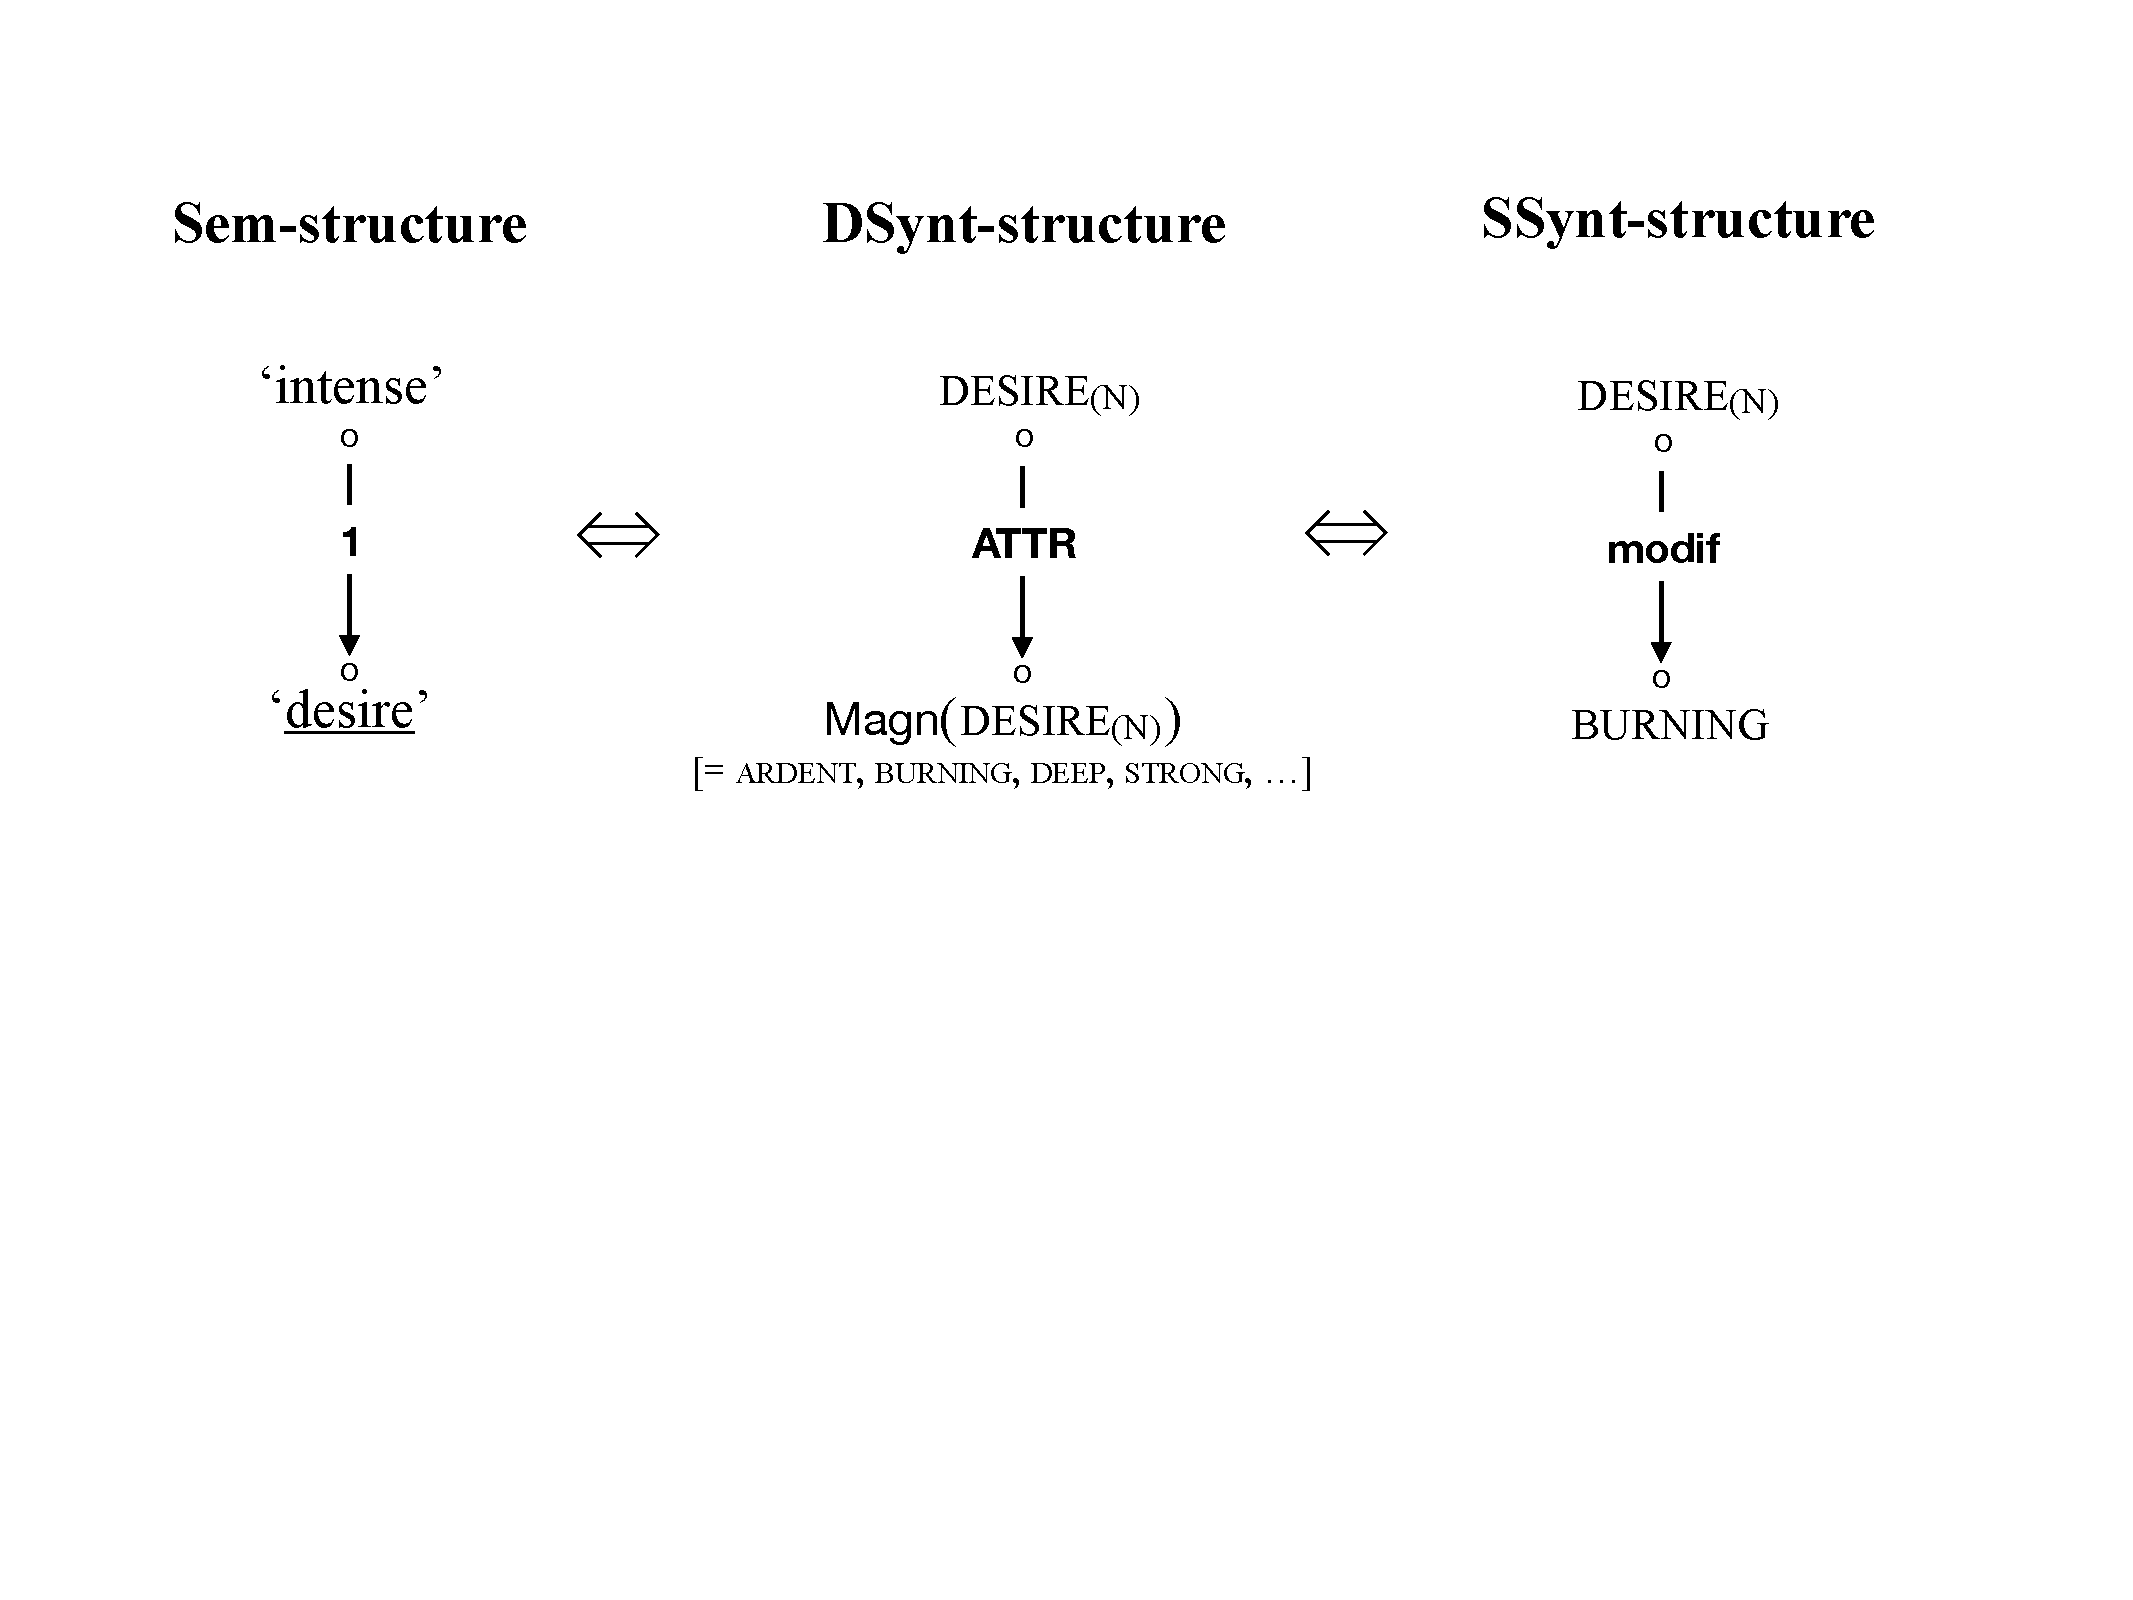
\includegraphics[width=12cm]{Fig/NotionLF/LFDSyntStruct.pdf}
\caption{\lf{Magn} in the DSyntS of the phrase \textit{burning desire}}\label{fig:LFDSyntStruct}
\end{figure}

\figref{fig:LFDSyntStruct} shows as well that, in linguistic representations, LFs appear only in DSyntSs. Being a lexical element in DSyntS, an LF has its own combinatorial properties, in particular, a deep part of speech\index[notion]{part of speech [PoS]!deep \tld} (see \sectref{sec:PofS}, p.\thinspace\pageref{sec:PofS}).

LFs fulfill two tasks in deep syntax: correct lexical selection (\sectref{sec:LFAndLexicalization}) and DSynt-paraphrasing (\sectref{sec:LFStandardParaphrasing}).

\subsubsection{LFs and lexical selection}\label{sec:LFAndLexicalization}

\notion{Lexical selection}\index[notion]{lexical selection|emph} is an important part of what is known as \notion{lexicalization}\index[notion]{lexicalization (in speech production)|emph} in speech production\index[notion]{speech!\tld\ production} -- e.g., in psycholinguistics\index[notion]{psycholinguistics} research \parencite{KempenHuijbers1983} and in computer text generation \parencite{Stede1994}.

Under lexical selection\index[notion]{lexical access\slashs{}selection}, LFs ensure correct choices in case a lexical unit has to be selected contingent upon another lexical unit in the same utterance.

Thus, \figref{fig:LFDSyntStruct} above represents the following steps in lexicalization:

\begin{enumerate}

\item At the Sem-level, the semanteme `intense' is identified as a constrained meaning\index[notion]{meaning!constrained \tld} (\sectref{sec:LFDefinitionNotion}, p.\thinspace\pageref{txt:constrainedMeaning}), to be lexically expressed as function of the expression of the semanteme `desire'.

\item At the DSynt-level, the semanteme `intense' is expressed by (the name of) the LF \lf{Magn}. This LF is applied to the lexeme \textsc{desire}\tsub{(N)}: the application \lfappl{Magn}{\textsc{desire}\tsub{(N)}} represents a constrained lexical choice, more precisely, a set of the usable syntactic modifiers of \textsc{desire}\tsub{(N)}, which express the semanteme `intense'.

\item At the SSynt-level, the lexical selection is completed: the lexeme \textsc{burning} is introduced as a modifier of \textsc{desire}\tsub{(N)}; this is done on the basis of the lexical entry\index[notion]{lexical entry} of \textsc{desire}\tsub{(N)}, where the value of the application \lfappl{Magn}{\textsc{desire}\tsub{(N)}} is specified.

\end{enumerate}

\subsubsection{LFs and paraphrasing}\label{sec:LFStandardParaphrasing}

A vital feature of natural languages is their ability to express, in a general case, a given meaning by a large set of quasi-synonymous utterances, i.e., \notion{paraphrases}\index[notion]{paraphrase|emph}, as shown in \figref{fig:paraphPotential}.

\begin{figure}

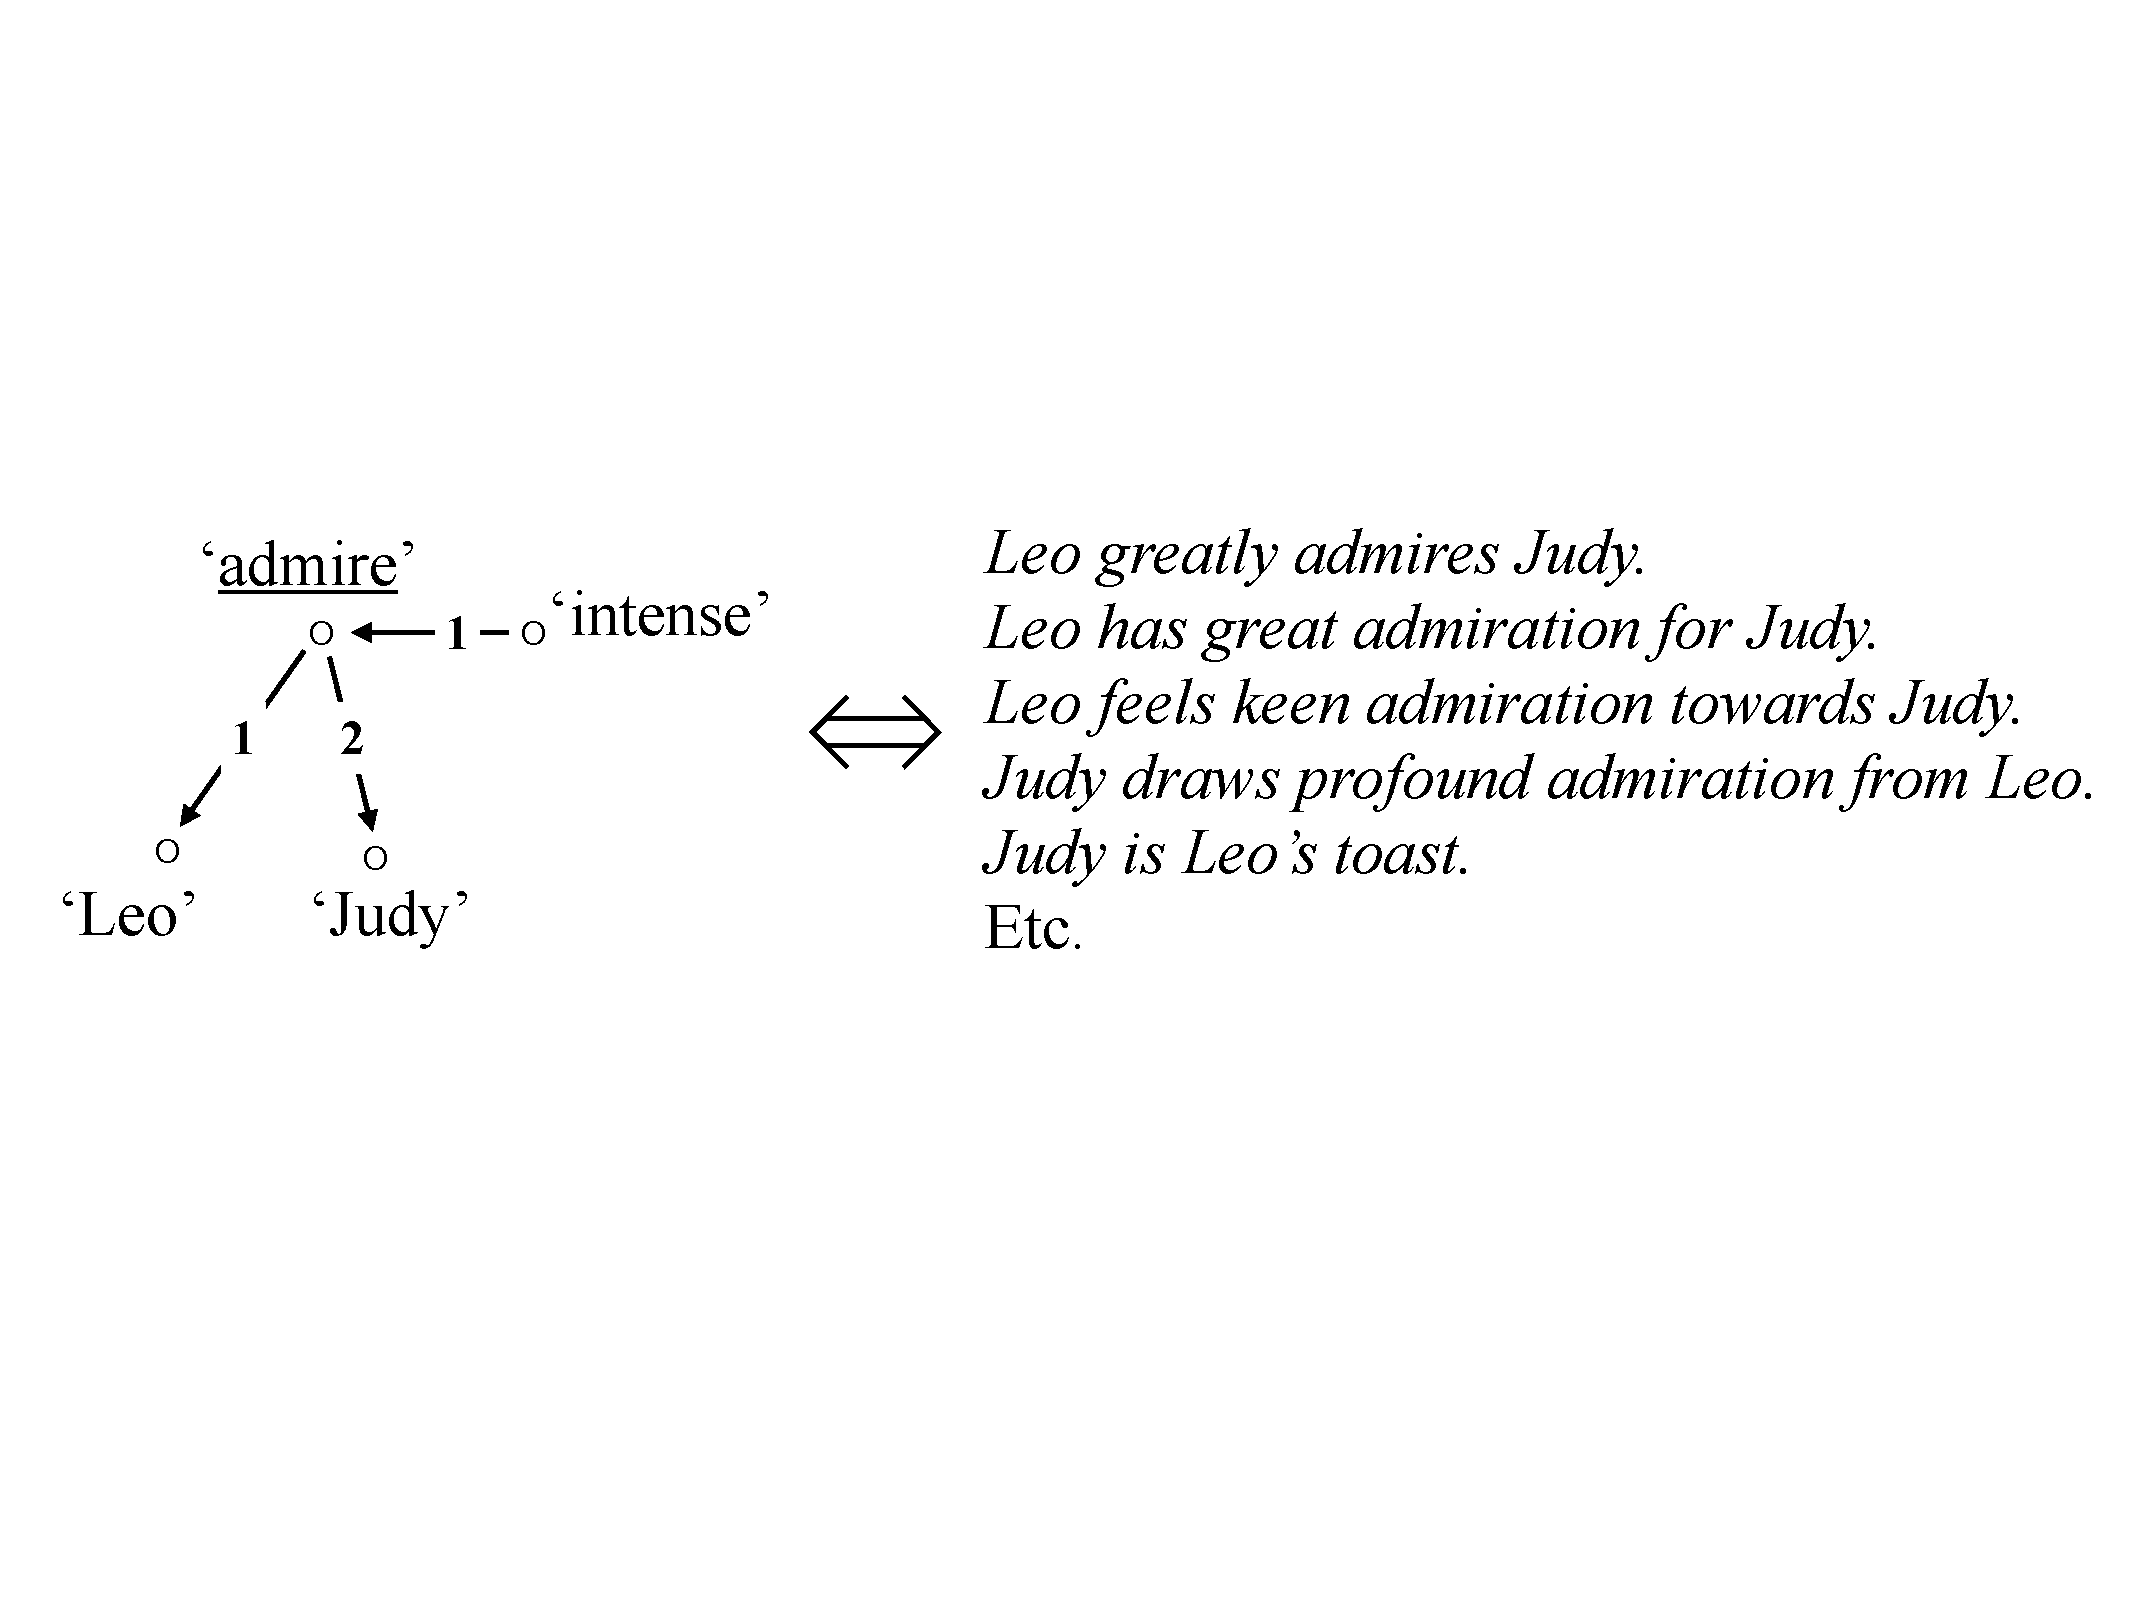
\includegraphics[width=11cm]{Fig/NotionLF/ParaphrasesIllustr.pdf}
\caption{Paraphrasing potential of a natural language}\label{fig:paraphPotential}
\end{figure}

This is but a modest illustration of what a natural language can do with regard to paraphrasing: a natural language is a paraphrasing device \parencite[Ch.~2]{Melcuk2012a-e}. Paraphrasing as such is not often used in actual speech production\index[notion]{speech!\tld\ production} -- only in specific situations: editing a text, rephrasing for better explanation, etc. However, the paraphrasing power\index[notion]{paraphrase!paraphrasing power of languages} of a language offers, at any given stage of speech production\index[notion]{speech!\tld\ production}, multiple alternatives that enable the Speaker\index[notion]{Speaker, the} to speak fluently. When speaking a second language, a person generally doesn't master the same paraphrasing wealth and therefore production can be slowed down or outright blocked.

The system of standard LFs\index[notion]{lexical function!system of standard \tlds}\index[notion]{system of standard LFs} plays a core role in the use of language, because it is in terms of LFs that \notion{deep-syntactic paraphrasing rules}\index[notion]{paraphrase!deep-syntactic paraphrasing rule|emph} are formulated. Since LFs are language-universal\index[notion]{language-universal} (see above, p.\thinspace\pageref{sec:universality}), the resulting system of paraphrasing rules is also universal. Such a paraphrasing system is described in \textcite[141--176]{Melcuk1974}, \textcite[Ch.~6]{Milicevic2007} and \textcite[Ch.~9]{Melcuk2013c-e}. Here, we limit ourselves to citing two paraphrasing rules: \textbf{R\tsub{\lf{Mult}}} and \textbf{R\tsub{\lf{Oper$_\text{1}$}}}.

\begin{center}
\APolbox{4.8cm}{%
\textbf{R\tsub{\lf{Mult}}:}\quad L\tsub{(N)\textsc{pl}}\enskip{\small $\equiv$}\enskip\lfappl{Mult}{L\tsub{(N)}}\tsub{\textsc{sg}}
}
\end{center}\phantomsection\label{txt:RParaphMult}\index[notion]{paraphrase!deep-syntactic paraphrasing rule!\textbf{R\tsub{\lf{Mult}}}|emph}\index[lf]{Mult@\lf{Mult}}

This rule describes the universal semantic equivalence between a plural noun L\tsub{(N)\textsc{pl}} and the corresponding collective noun \lfappl{Mult}{L} -- \chapref{chap:paraLFs}, [\ref{lf:Mult}], p.\thinspace\pageref{lf:Mult}; for instance:

\begingroup
\small

\ex. \begin{tabular}[t]{l c l}
     \textit{workers} & {\footnotesize $\cong$} & \textit{workforce} \\
     \textit{lies} & {\footnotesize $\cong$} & \textit{bunch of lies} \\
     \end{tabular}

\endgroup

Note that such equivalences hold for a specific meaning of the nominal plural: `collective of \lfgp{Ns}'. \lfappl{Mult}{L} itself is in the singular, as stated in the rule \textbf{R\tsub{\lf{Mult}}}.

\begin{center}
\APolbox{7.2cm}{%
\textbf{R\tsub{\lf{Oper$_\text{1}$}}:} L\tsub{(V)}\enskip{\small $\equiv$}\enskip\lfappl{Oper\tsub{1}}{\lfappl{S\tsub{0}}{L\tsub{(V)}}}\thinspace\syntRel{II}\thinspace\lfappl{S\tsub{0}}{L\tsub{(V)}}
}
\end{center}\phantomsection\label{txt:RParaphOper1}\index[notion]{paraphrase!deep-syntactic paraphrasing rule!\textbf{R\tsub{\lf{Oper$_\text{1}$}}}|emph}\index[lf]{S0@\lf{S\tsub{0}}}\index[lf]{Operi@\lf{Oper\tsub{i}}!\lf{Oper\tsub{1}}}

This rule describes the universal semantic equivalence between a verb L\tsub{(V)} and the verbal collocation consisting of (i)~the \lf{S\tsub{0}} nominalization of L\tsub{(V)} (\chapref{chap:paraLFs}, [\ref{lf:S0}], p.\thinspace\pageref{lf:S0}) and (ii)~an \lf{Oper\tsub{1}} support verb of this nominalization (\chapref{chap:syntLFs}, [\ref{lf:Oper-i}], p.\thinspace\pageref{lf:Oper-i}). For instance:

\begingroup
\small

\ex. Leo \emph{admires} Judy.\enskip{\footnotesize $\equiv$}\enskip Leo \emph{has admiration} for Judy.

\endgroup

\subsubsection{Actantial subscripts in simple standard LFs}\label{sec:actSubsSimpleLF}

Actantial subscripts\index[notion]{actantial subscript|emph} to LF names have frequently appeared in the preceding text. An explanation of their interpretation is supplied here for the names of simple standard LFs. The corresponding explanation concerning the names of LFs in combinations\index[notion]{lexical function!\tld\ combination} is provided in \sectref{sec:actSubsLFCombinations} (p.\thinspace\pageref{sec:actSubsLFCombinations}).

In the general case of an application \lfappl{f\tsub{i}}{L} where \lf{f\tsub{i}} is a simple LF, the subscript ``\tsub{\lf{i}}'' refers to the DSyntA\thinspace\syntDname{i} of L. Here are two illustrations, with LFs \lf{S\tsub{2}}\index[lf]{Si@\lf{S\tsub{i}}!\lf{S\tsub{2}}} (\chapref{chap:paraLFs}, [\ref{lf:S-i}], p.\thinspace\pageref{lf:S-i}) and \lf{Func\tsub{3}}\index[lf]{Funci@\lf{Func\tsub{i}}!\lf{Func\tsub{3}}} (\chapref{chap:syntLFs}, [\ref{lf:Func-i}], p.\thinspace\pageref{lf:Func-i}).

\begingroup
\small

\ex. \a. \begingroup\setlength{\tabcolsep}{2pt}
\begin{tabular}[t]{ l l l }
\lfappl{S\tsub{\textbf{2}}}{\textit{eat} \lfgp{`X eats \textbf{Y}'}} & = & \textit{food} \\
\end{tabular}\endgroup
      \b. \begingroup\setlength{\tabcolsep}{2pt}
\begin{tabular}[t]{ l l l }
\lfappl{Func\tsub{\textbf{3}}}{\textit{ultimatum} \lfgp{`X's ultimatum to Y to do \textbf{Z} before time T'}} & = & \textit{call}\tsub{(V)} \lfgp{\textit{for} N\tsub{Z}} \\
\multicolumn{3}{l}{Ex.: \textit{The ultimatum calls}\tsub{\lfappl{Func$_\text{3}$}{\textit{ultimatum}}} \textit{for the release}\tsub{Z} \textit{of prisoners.}} \\
\end{tabular}\endgroup

\endgroup

However, there are at least three special cases of LFs where the interpretation of actantial subscripts is not straightforward:
 
 \begin{itemize}
 
 \item \lf{Adv\tsub{(i)}}\index[lf]{Advi@\lf{Adv\tsub{i}}!\lf{Adv\tsub{(i)}}}, which stands for absolutive adverbials\index[notion]{adverb!absolutive \tld ial} (such as \textit{in the presence of}) -- see \chapref{chap:paraLFs}, [\ref{lf:Adv-i}], Comment~2, p.\thinspace\pageref{para:comment2Advi};
 
 \item \lf{Sympt\tsub{ijk}}\index[lf]{Symptijk@\lf{Sympt\tsub{ijk}}}, which describes somatic phrasemes\index[notion]{phraseme!somatic \tld} of psychological or physiological states -- see \chapref{chap:syntLFs}, [\ref{lf:Sympt-ijk}], p.\thinspace\pageref{lf:Sympt-ijk};

\item \lf{Caus}\index[lf]{Caus@\lf{Caus}}, \lf{Liqu}\index[lf]{Liqu@\lf{Liqu}} and \lf{Perm}\index[lf]{Perm@\lf{Perm}}, which stand for verbs of causing\index[notion]{lexical function!\tld\ of causing} -- see \chapref{chap:syntLFs}, \sectref{sec:collocCausatif}.
 
 \end{itemize}

\section{Two major classes of simple standard LFs}\label{sec:LFParaSynt}\index[notion]{lexical function!paradigmatic vs. syntagmatic \tlds|emph}

LFs are divided in two classes, based on the two functional axes of natural languages \parencite[Part~2, Ch.~V]{Saussure1972}:

\begin{itemize}

\item the \notion{paradigmatic axis}\index[notion]{paradigmatic!\tld\ axis}, on which the Speaker\index[notion]{Speaker, the} performs the \emph{selection} of linguistic units to be used;

\item the \notion{syntagmatic axis}\index[notion]{syntagmatic!\tld\ axis}, on which the Speaker performs the \emph{combination} of selected linguistic units into higher-level units.

\end{itemize}

These two axes and the corresponding linguistic operations (selection vs. combination) determine the two classes of LFs: paradigmatic LFs (\sectref{sec:classeFLParadigmatiques}) and syntagmatic LFs (\sectref{sec:classeFLSyntagmatiques}).%\footnote{In the process of text production the operations of selection and combination intermingle: a particular selection of a linguistic unit specifies the conditions for eventual combinations, and a particular combination can require an alternative selection.}

\subsection{Paradigmatic LFs}\label{sec:classeFLParadigmatiques}

The application\index[notion]{application of an LF}\index[notion]{lexical function!application of a \tld} of a \notion{paradigmatic LF}\index[notion]{lexical function!paradigmatic \tld|emph}\index[notion]{paradigmatic!\tld\ lexical function|emph} to a lexical unit L returns as value\index[notion]{lexical function!value of a \tld}\index[notion]{value of an LF} a set of lexical entities of which each element L′ stands in a particular paradigmatic relation to L -- i.e., L′ is a possible substitute for L in the text. More precisely, L′ is a \notion{semantic derivative}\index[notion]{derivative!semantic \tld|emph}\index[notion]{semantic!\tld\ derivative|emph} of L. 

\phantomsection\label{def:semanticDerivative}\begin{notiondefinition}{semantic derivative}
A \notion{semantic derivative} of lexical unit L is a lexical entity L′ whose meaning `L′' includes `L' such that \\*[2pt]
\setlength{\tabcolsep}{.5pt}\begin{tabular}{ p{0.2cm} >{\raggedright\arraybackslash}p{11.1cm} }
\SpecDiff & the semantic difference `$\sigma$' $=$ `L′\verythinspace\textminus\verythinspace L' is found in a large enough number of lexical pairs of the language -- i.e., `$\sigma$' is regular\index[notion]{regularity}; \\
\SpecDiff & the language has dedicated means for expressing `$\sigma$' -- e.g., morphological means. \\[3pt]
\end{tabular}

\noindent
L is called the \notion{base of the derivative} L′.
\end{notiondefinition}\index[notion]{base!\tld\ of a derivative}\index[notion]{derivative!base of a \tld}\index[notion]{morphology!morphological means}

As anticipated by the above definition, there is a particular case of semantic derivative: \notion{morphological derivative}\index[notion]{derivative!morphological \tld}\index[notion]{morphology!morphological derivative}.

\begin{notiondefinition}{morphological derivative}
A \notion{morphological derivative} of lexical unit L is a semantic derivative L′ of L such that \\*[2pt]
\setlength{\tabcolsep}{.5pt}\begin{tabular}{ p{0.2cm} >{\raggedright\arraybackslash}p{11.1cm} }
\SpecDiff & the semantic difference `L′\verythinspace\textminus\verythinspace L' is expressed by a morphological means. \\
\end{tabular}
\end{notiondefinition}\index[notion]{morphology!morphological means}

A typical case of derivatives is that of \notion{Agent noun}\index[notion]{Agent (semantic role)!\tld\ noun}\index[notion]{semantic!\tld\ role}, or more precisely, the name for the first semantic actant\index[notion]{actant!semantic \tld\ [SemA]}\index[notion]{semantic!\tld\ actant [SemA]} [SemA~\syntDname{1}] `X' of L. Here are a few illustrations:

\begingroup
\small

\ex.\label{ex:illustrationsAgent} \begingroup\setlength{\tabcolsep}{2pt}
\begin{tabular}[t]{ l l >{\raggedright\arraybackslash}p{7.5cm} }
\textit{support}\tsub{(V)} & \lexRel{\lf{Agent noun}} & \textit{supporter} {\footnotesize `X who supports'} \\
\textit{agression} & \lexRel{\lf{Agent noun}} & \textit{agressor} {\footnotesize `X who commits an agression'} \\
\textit{congress} & \lexRel{\lf{Agent noun}} & \textit{congressman}\slashs\textit{congresswoman} {\footnotesize `X who is a member of a country's congress'} \\
\textit{boring} & \lexRel{\lf{Agent noun}} & \textit{bore}\tsub{(N)} {\footnotesize `X who is boring'} \senseex{He is an awful bore.} \\
\textit{account}\tsub{(N)} & \lexRel{\lf{Agent noun}} & \textit{account holder} {\footnotesize `X who has a bank account'} \\
\textit{steal}\tsub{(V)} & \lexRel{\lf{Agent noun}} & \textit{thief} {\footnotesize `X who steals'} \\
\textit{annoying} & \lexRel{\lf{Agent noun}} & \uslabel{vulgar} \idiom{\textit{pain in the ass}} {\footnotesize `X that is annoying'} \\*
\textit{heal} & \lexRel{\lf{Agent noun}} & \textit{remedy}\tsub{(N)} {\footnotesize `X that heals'} \\
\end{tabular}\endgroup

\endgroup

Among these semantic derivatives, the first four are also morphological derivatives\index[notion]{derivative!morphological \tld}\index[notion]{morphology!morphological derivative}.

Semantic derivation is described by paradigmatic LFs in the following way:

\begin{itemize}

\item a given paradigmatic LF \lf{f} specifies a particular family of semantic derivatives that express the meaning \sigmaF;

\item it takes as arguments the bases of derivatives;

\item it returns as values the derivatives themselves.

\end{itemize}

For instance, the semantic derivation of Agent\index[notion]{Agent (semantic role)}\index[notion]{semantic!\tld\ role} nouns mentioned above is described by the paradigmatic LF \lf{S\tsub{1}}\index[lf]{Si@\lf{S\tsub{i}}!\lf{S\tsub{1}}} with the meaning `somebody who\slashs{}something that ...' (\chapref{chap:paraLFs}, [\ref{lf:S-i}], p.\thinspace\pageref{lf:S-i}). For  the illustrations \ref{ex:illustrationsAgent}, it is encoded as in \ref{ex:illustrationsAgentEncoding}:

\begingroup
\small

\ex.\label{ex:illustrationsAgentEncoding} \begingroup\setlength{\tabcolsep}{2pt}
\begin{tabular}[t]{ l l >{\raggedright\arraybackslash}p{7cm} }
\lfappl{S\tsub{1}}{\textit{support}\tsub{(V)}} & = & \textit{supporter} \\
\lfappl{S\tsub{1}}{\textit{agression}} & = & \textit{agressor} \\
\lfappl{S\tsub{1}}{\textit{congress}} & = & \textit{congressman}\textbf{,} \textit{congresswoman} \\
\multicolumn{3}{ l }{etc.} \\
\end{tabular}\endgroup

\endgroup

\paragraph*{Remark on the LF \lf{Syn}.}\label{par:remarkOnSyn}

The LF \lf{Syn}\index[lf]{Syn@\lf{Syn}} `synonym' (\chapref{chap:paraLFs}, [\ref{lf:Syn}], p.\thinspace\pageref{lf:Syn}) occupies a special place among paradigmatic LFs. It models a particular case of the most important relation underlying the functioning of natural languages: \notion{synonymy in the broad sense}\index[notion]{synonymy!\tld\ in the broad sense}, i.e., semantic equivalence between linguistic expressions. Consequently, \lf{Syn} underlies the simplest paraphrasing rule\index[notion]{paraphrase!deep-syntactic paraphrasing rule}:

\begin{center}
\APolbox{3.3cm}{%
\textbf{R\tsub{\lf{Syn}}:}\quad L\enskip{\small $\equiv$}\enskip\lfappl{Syn}{L}\label{ex:regleParaphrasageSyn}
}
\end{center}\label{txt:RSyn}\index[notion]{paraphrase!deep-syntactic paraphrasing rule!\textbf{R\tsub{\lf{Syn}}}|emph}

Note that all paraphrasing rules -- e.g., rules \textbf{R\tsub{Mult}}\index[notion]{paraphrase!deep-syntactic paraphrasing rule!\textbf{R\tsub{\lf{Mult}}}} and \textbf{R\tsub{\lf{Oper$_\text{1}$}}}\index[notion]{paraphrase!deep-syntactic paraphrasing rule!\textbf{R\tsub{\lf{Oper$_\text{1}$}}}} (\sectref{sec:LFStandardParaphrasing}, p.\thinspace\pageref{txt:RParaphMult}) -- establish the synonymy\index[notion]{synonymy} relations between linguistic expressions. Even more importantly, the Meaning-Text approach\index[notion]{Meaning-Text!\tld\ approach} is built on the notion of \notion{Meaning}\index[notion]{meaning!Meaning \lfgp{with a capital \textit{M}}} (written with a capital \textit{M}), which is the invariant of a set of paraphrases, i.e., synonymous expressions \parencites[10--11]{Melcuk1974}[44--45]{Melcuk2012a-e}[102--103]{MelcukMilicevic2014a}.

\subsection{Syntagmatic LFs}\label{sec:classeFLSyntagmatiques}

The application\index[notion]{application of an LF}\index[notion]{lexical function!application of a \tld} of a \notion{syntagmatic LF}\index[notion]{lexical function!syntagmatic \tld|emph}\index[notion]{syntagmatic!\tld\ lexical function|emph} to a lexical unit L\tsub{1} returns as value a set of lexical entities of which each element L\tsub{2} stands in a particular syntagmatic (i.e., cooccurrence\index[notion]{cooccurrence, restricted}) relation with L\tsub{1}. More precisely, L\tsub{2} forms a \notion{collocation}\index[notion]{collocation|emph} with L\tsub{1}.\footnote{\phantomsection\label{fn:NatureCollocates}The following definition would necessitate fine-tuning. In practice, instances of some sort of double-shot collocations can be found, where the collocate L\tsub{2} is not a lexical unit but is itself a collocation. For instance, the phraseme \textit{under the effect of alcohol} has all appearances of being a double-shot collocation, where \textsc{alcohol} is the base and \textit{under the effect} is itself a collocation with \textsc{effect}\tsub{(N)} as its base. For a description of \textit{under the effect} in terms of the LF \lf{A\tsub{2}}, see \chapref{chap:paraLFs}, [\ref{lf:A-i}], p.\thinspace\pageref{txt:A2UnderTheEffect}; for a description of \textit{under the effect of alcohol} in terms of the LF \lf{Propt\tsub{1}}, see \chapref{chap:syntLFs}, [\ref{lf:Propt-i}], p.\thinspace\pageref{txt:Propt1UnderTheEffectOfAlcohol}. Note that the LF \lf{Sympt\tsub{ijk}} is often used to encode phrasemes that seem like double-shot collocations -- see \chapref{chap:syntLFs}, [\ref{lf:Sympt-ijk}], p.\thinspace\pageref{lf:Sympt-ijk}.}\index[notion]{collocation!double-shot \tld|emph}\index[lf]{Ai@\lf{A\tsub{i}}!\lf{A\tsub{2}}}\index[lf]{Propti@\lf{Propt\tsub{i}}!\lf{Propt\tsub{1}}}\index[lf]{Symptijk@\lf{Sympt\tsub{ijk}}}

\phantomsection\label{def:collocation}\begin{notiondefinition}{collocation}
A \notion{collocation} is a compositional phraseme\index[notion]{phraseme} consisting, prototypically, of two lexical units L\tsub{1} and L\tsub{2} such that \\*
\setlength{\tabcolsep}{.5pt}\begin{tabular}{ p{0.2cm} >{\raggedright\arraybackslash}p{11cm} }
\SpecDiff & L\tsub{1} is selected by the Speaker\index[notion]{Speaker, the} freely, i.e., independently of any other lexical choice; \\
\SpecDiff & L\tsub{2} is selected by the Speaker to express a particular meaning \sigmaF\ in combination with L\tsub{1} as a function of L\tsub{1}. \\[3pt]
\multicolumn{2}{l}{L\tsub{1} is called the \notion{base of the collocation} and L\tsub{2}, its \notion{collocate}.} \\[3pt]
\end{tabular}

\noindent
\remark{Examples.}In the collocation \textit{deep feeling}, \textit{feeling} is the base and \textit{deep}, the collocate; in \textit{pay a visit}, \textit{visit} is the base and \textit{pay}, the collocate.
\end{notiondefinition}\index[notion]{base!\tld\ of a collocation|emph}\index[notion]{collocation!base of a \tld|emph}\index[notion]{collocation!collocate of a \tld|emph}

An emblematic case of collocation is that of intensification; here are three examples where collocates are italicized:

\begingroup
\small

\ex.\label{ex:collocationIntensification} \a. \emph{nagging} doubt
     \b. Thanks \emph{a million}!
     \c. drink \emph{\idiom{like a sponge}}

\endgroup

Syntagmatic LFs take as arguments lexical units that are bases of collocations and return as values lists of corresponding collocates. For instance, intensification collocations are accounted for by the syntagmatic LF \lf{Magn}\index[lf]{Magn@\lf{Magn}} (\chapref{chap:syntLFs}, [\ref{lf:Magn}], p.\thinspace\pageref{lf:Magn}), so that collocations given in \ref{ex:collocationIntensification} are described as \ref{ex:collocationIntensificationDescr}:

\begingroup
\small

\ex.\label{ex:collocationIntensificationDescr} \begingroup\setlength{\tabcolsep}{2pt}
\begin{tabular}[t]{ l l >{\raggedright\arraybackslash}p{8cm} }
\lfappl{Magn}{\textit{doubt}\tsub{(N)}} & = & \textit{strong} \textbf{<} \textit{gnawing}\textbf{,} \textit{nagging}\textbf{;} \textit{lingering} \\
\lfappl{Magn}{\textit{Thanks!}} & = & \textit{a lot} \lfconstr{postposed}\textbf{,} \textit{a million} \lfconstr{postposed} \\
\lfappl{Magn}{\textit{drink}\tsub{(V)}} & = & \textit{heavily}\textbf{,} \idiom{\textit{like a fish}}\textbf{,} \idiom{\textit{like a sponge}} \\
\end{tabular}\endgroup

\endgroup

\begin{furtherreading}
For more on the notion of collocation, see \textcite{Hausmann1979}, \textcite{Wanner1996}, \textcite{Melcuk1998} and \textcite[Ch.~6]{Melcuk2023a}.
\end{furtherreading}

\paragraph*{Semantic target of a syntagmatic LF.}\label{txt:targetOfSyntLF}

For a full [=~semantically loaded] syntagmatic LF such as \lf{Magn},\footnote{By contrast, support verb LFs (see \chapref{chap:syntLFs}, \sectref{sec:verbeSupport}) are examples of semantically empty syntagmatic LFs.} the meaning of \lfappl{f}{L}, i.e. the meaning of L's collocate that is returned as value, necessarily applies to a component of L's lexicographic definition\index[notion]{definition!lexicographic \tld} \parencite{IordanskajaPolguere2005}. Let us call such a component the (semantic) \notion{target} of the LF\index[notion]{target of an LF|emph}\index[notion]{lexical function!target of a \tld|emph}\index[notion]{lexical function!\tld\ and components of a lexicographic definition|see{target of an LF}}.

In most cases, the LF target in L's definition is its central component\index[notion]{definition!central component of a \tld}\index[notion]{component of a definition!central \tld} and need not be explicitly indicated in the encoding of the LF. If, however, the target is not the central component, it must be specified as a subscript to the LF name; for instance, for \lf{Magn}:

\begingroup
\small

\ex. \begingroup\setlength{\tabcolsep}{2pt}
\begin{tabular}[t]{ l l >{\raggedright\arraybackslash}p{7cm} }
\lfappl{Magn}{\textit{earthquake}} & = & \textit{powerful}\textbf{,} \textit{strong} \textbf{<} \textit{major}\textbf{,} \textit{massive} \\*
\lfappl{Magn\tsub{`damage'}}{\textit{earthquake}} & = & \textit{catastrophic}\textbf{,} \textit{devastating}\textbf{;} \textit{deadly} \\*[3pt]
\multicolumn{3}{>{\raggedright\arraybackslash}p{10cm}}{\remark{Note.}The approximate definition of \textsc{earthquake} is `sudden shaking of the Earth's surface, able to cause serious \emph{damage} around location Y'.} \\
\end{tabular}\endgroup

\endgroup

Follows an illustration for the verbal syntagmatic LF \lf{Real\tsub{i}}\index[lf]{Reali@\lf{Real\tsub{i}}} (see \chapref{chap:syntLFs}, [\ref{lf:Real-i}], p.\thinspace\pageref{lf:Real-i}):

\begingroup
\small

\ex. \begingroup\setlength{\tabcolsep}{2pt}
\begin{tabular}[t]{ l l >{\raggedright\arraybackslash}p{7cm} }
\lfappl{Real\tsub{1,`hostile action'}}{\textit{anger}\tsub{(N)}} & : & \textit{vent} \lfgp{A\tsub{(poss)X} \tld\ \textit{on} N\tsub{Y}} \\*
\lfappl{Real\tsub{1,`loss of self-control'}}{\textit{anger}\tsub{(N)}} & : & \idiom{\textit{be beside oneself}} \lfgp{\textit{with} \tld}\\
\end{tabular}\endgroup

\endgroup

The lexical entry for \textsc{anger}\tsub{(N)} in the Appendix (p.\thinspace\pageref{chap:appendix1}) presents more examples of the same kind.

\subsection{Paradigmatic and syntagmatic LFs in contact}\label{sec:interconnexionParaSynt}\index[notion]{lexical function!paradigmatic vs. syntagmatic \tlds}

Both classes of LFs -- paradigmatic and syntagmatic ones -- are designed to fulfill the same role, namely, to specify lexical expressions of constrained meanings\index[notion]{meaning!constrained \tld} (\sectref{sec:LFDefinitionNotion}, p.\thinspace\pageref{txt:constrainedMeaning}). Therefore, they are expected to be frequently intertwined; and in fact, they are. Their interactions are of two kinds: with respect to the values they return (\sectref{sec:quidProQuoValues}) and with respect to their use in linguistic description (\sectref{sec:interactionLFs}).

\subsubsection{Quid pro quo in LF values}\label{sec:quidProQuoValues}\index[notion]{lexical function!value of a \tld}\index[notion]{value of an LF}

The paradigmatic LFs express derivational meanings and are supposed to return semantic derivatives\index[notion]{derivative!semantic \tld}\index[notion]{semantic!\tld\ derivative} of their arguments; the syntagmatic LFs express collocational meanings\index[notion]{meaning!collocational \tld} and are supposed to return collocates\index[notion]{collocation!collocate of a \tld} of their arguments.

\begin{soundboxnotitle}
However, there is no airtight partition between the two classes of paradigmatic vs. syntagmatic LFs with respect to the lexical nature of their values.
\end{soundboxnotitle}

This happens because both types of LFs do essentially the same job: they supply an appropriate expression means for a meaning to be added to the meaning of the base (of a derivative or of a collocation). The fundamental difference between the two types of LFs in this respect is as follows: for paradigmatic LFs, these means tend to be affixal\index[notion]{affix} -- at least, in \notion{Standard Average European} [SAE]\index[notion]{Standard Average European [SAE] language|emph}\index[notion]{SAE|see{Standard Average European [SAE] language}}\footnote{Roughly, SAE languages are Germanic, Romance and Slavic languages \parencite{Whorf1941}.} languages; for the syntagmatic LFs, the expressive means are normally separate lexical units. As a result, the values of the paradigmatic LFs are rather synthetic, and those of the syntagmatic LFs, rather analytic. But, as is always the case with natural languages, this distinction is not implemented 100\% systematically: there are analytic values of paradigmatic LFs and synthetic values of syntagmatic LFs.

\paragraph*{Analytic values of paradigmatic LFs.}\label{par:analyticValuesParaLFs}\index[notion]{derivative!analytic semantic \tld}\index[notion]{lexical function!analytic value of a \tld}\index[notion]{value of an LF!analytic \tld}

A paradigmatic LF \lf{f} applied to a lexical unit L can return (instead of a one-piece semantic derivative) a collocation of L, which is, so to speak, an analytic semantic derivative of L. Such is the case of two previously mentioned examples: the analytic value \textit{account holder} for \lfappl{S\tsub{1}}{\textit{account}\tsub{(N)}} and \textit{in doubt} for \lfappl{A\tsub{1}}{\textit{doubt}\tsub{(N)}}; see \Next:

\begingroup
\small

\ex. \begingroup\setlength{\tabcolsep}{2pt}
\begin{tabular}[t]{ l l >{\raggedright\arraybackslash}p{7cm} }
\lfappl{S\tsub{1}}{\textit{account}\tsub{(N)}} & = & \tld\ \textit{holder} \\*
\lfappl{A\tsub{1}}{\textit{doubt}\tsub{(N)}} & = & \textit{doubtful}\textbf{,} \textit{in} \tld \\
\end{tabular}\endgroup

\endgroup\index[lf]{Si@\lf{S\tsub{i}}!\lf{S\tsub{1}}}\index[lf]{Ai@\lf{A\tsub{i}}!\lf{A\tsub{1}}}

This phenomenon is quite typical of some paradigmatic LFs, in particular of the collective \lf{Mult}\index[lf]{Mult@\lf{Mult}} (\chapref{chap:paraLFs}, [\ref{lf:Mult}], p.\thinspace\pageref{lf:Mult}):

\begingroup
\small

\ex. \begingroup\setlength{\tabcolsep}{2pt}
\begin{tabular}[t]{ l l >{\raggedright\arraybackslash}p{7cm} }
\lfappl{Mult}{\textit{fish}\tsub{(N)}} & = & \textit{school of} \tld \\
\lfappl{Mult}{\textit{attack}\tsub{(N)}} & = & \textit{spate of} \tld\textit{s} \\*
\lfappl{Mult}{\textit{activity}} & = & \textit{flurry of} \tld \\
\end{tabular}\endgroup

\endgroup

\paragraph*{Synthetic [= fused] values of syntagmatic LFs.}\label{par:fusedValuesSyntLFs}

A syntagmatic LF \lf{f} applied to L can return -- instead of a collocate of L -- a semantic derivative\index[notion]{derivative!semantic \tld}\index[notion]{semantic!\tld\ derivative} of L: a lexical unit that synthetically expresses the linguistic union\index[notion]{linguistic union \lfgp{operation}} of the meanings `L' and \sigmaF. For instance, in the case of the attenuation LF \lf{AntiMagn}\index[lf]{AntiMagn@\lf{AntiMagn}}\index[lf]{Magn@\lf{Magn}!AntiMagn@\lf{AntiMagn}} (antonym\index[notion]{antonym} of \lf{Magn}):

\begingroup
\small

\ex. \begingroup\setlength{\tabcolsep}{2pt}
\begin{tabular}[t]{ l l >{\raggedright\arraybackslash}p{7cm} }
\lfappl{AntiMagn}{\textit{rain}\tsub{(N)}} & = & \textit{light}\textbf{,} \fused\textit{drizzle}\tsub{(N)} \lfgp{$\cong$\enskip\textit{light rain}} \\
\end{tabular}\endgroup\label{ex:AntiMagnRAIN}

\endgroup

The noun \textsc{drizzle}\tsub{(N)} is a semantic derivative of \textsc{rain}\tsub{(N)}, namely, a richer synonym \lf{Syn\tsub{$\supset$}}\index[lf]{Syn@\lf{Syn}!\lf{Syn\tsub{$\supset$}}} rather than a genuine collocate, such as \textsc{light}\tsub{(Adj)}.

The phenomenon under consideration is called \notion{fusion}\index[notion]{fusion|emph}, and the corresponding value is a \notion{fused value}\index[notion]{value of an LF!fused \tld|emph}\index[notion]{lexical function!fused value of a \tld|emph}. Fusion is indicated, as shown above, by the symbol ``\fused''\phantomsection\label{fusionFL}.

\subsubsection{Interaction of paradigmatic and syntagmatic LFs}\label{sec:interactionLFs}

\paragraph*{Cohabitation of LFs in paraphrasing rules.}\index[notion]{paraphrase!deep-syntactic paraphrasing rule}

Syntactic paraphrasing rules (cf. \sectref{sec:LFStandardParaphrasing}), which are crucial for the functioning of language, actively exploit both families of LFs, often making them collaborate within the same rule. This latter case is illustrated by rule \textbf{R\tsub{\lf{Oper$_\text{1}$}}}\index[notion]{paraphrase!deep-syntactic paraphrasing rule!\textbf{R\tsub{\lf{Oper$_\text{1}$}}}} (\sectref{sec:LFStandardParaphrasing}, p.\thinspace\pageref{txt:RParaphOper1}), which simultaneously uses the paradigmatic \lf{S\tsub{0}}\index[lf]{S0@\lf{S\tsub{0}}} and the syntagmatic \lf{Oper\tsub{1}}\index[lf]{Operi@\lf{Oper\tsub{i}}!\lf{Oper\tsub{1}}}.

\paragraph*{Semantic connections.}

A paradigmatic LF and a syntagmatic LF can show interesting semantic connections; here are two examples.

\begin{enumerate}

\item The paradigmatic LF \lf{S\tsub{1}}\index[lf]{Si@\lf{S\tsub{i}}!\lf{S\tsub{1}}} applied to a verb L means `somebody\slashs{}something that does L' -- L is, so to speak, what \lf{S\tsub{1}} is supposed to do;  and the syntagmatic LF \lf{Fact\tsub{0}}\index[lf]{Facti@\lf{Fact\tsub{i}}!\lf{Fact\tsub{0}}} applied to a noun L′ means `[L′] does what it is supposed to do'. From this it follows:

\begingroup
\small

\ex. \begingroup\setlength{\tabcolsep}{1.5pt}
\begin{tabular}[t]{ l c >{\raggedright\arraybackslash}p{1.5cm} >{\raggedright\arraybackslash}p{1.5cm} >{\raggedright\arraybackslash}p{1.8cm} c >{\raggedright\arraybackslash}p{1.4cm} }
%\midrule
\lfappl{S\tsub{1}}{L\tsub{(`action')}} & = & L′ & {\footnotesize implies}
& \lfappl{Fact\tsub{0}}{L′} & = &
\multicolumn{1}{>{\raggedright\arraybackslash}p{1.5cm}}{L\tsub{(`action')}} \\*[3pt]
%\midrule  \\*[-6pt]
\multicolumn{7}{l}{\remark{Examples:}} \\*
\lfappl{S\tsub{1}}{\textit{ski}\tsub{(V)}} & = & \textit{skier}
& {\footnotesize implies}
&  \lfappl{Fact\tsub{0}}{\textit{skier}} & = & \textit{ski}\tsub{(V)} \\*
\lfappl{S\tsub{1}}{\textit{sell}\tsub{(V)}} & = & \textit{seller}
& {\footnotesize implies}
&  \lfappl{Fact\tsub{0}}{\textit{seller}} & = & \textit{sell}\tsub{(V)} \\
\end{tabular}\endgroup\label{ex:paraImpliesSynt}

\endgroup

\item A modifying syntagmatic LF -- \lf{Magn}\index[lf]{Magn@\lf{Magn}}, \lf{Ver}\index[lf]{Ver@\lf{Ver}} or \lf{Bon}\index[lf]{Bon@\lf{Bon}} -- in case of fusion\index[notion]{fusion}\index[notion]{value of an LF!fused \tld} adds to L a meaning such that the resulting L′ can be considered a richer synonym \lf{Syn\tsub{$\supset$}}\index[lf]{Syn@\lf{Syn}!\lf{Syn\tsub{$\supset$}}} of L, \lf{Syn\tsub{$\supset$}} being a typical paradigmatic LF:

\begingroup
\small

\ex.\label{ex:FusedMagnAndRicherSyn}\begingroup\setlength{\tabcolsep}{1.5pt}
\begin{tabular}[t]{ l c >{\raggedright\arraybackslash}p{2.2cm} >{\raggedright\arraybackslash}p{1.5cm} >{\raggedright\arraybackslash}p{2.2cm} c >{\raggedright\arraybackslash}p{1.5cm} }
%\midrule
\lfappl{Magn}{L}
& = & \fused{}L′
& {\footnotesize implies}
& \lfappl{Syn\tsub{$\supset$}}{L} & = &
\multicolumn{1}{>{\raggedright\arraybackslash}p{1.5cm}}{L′} \\*[3pt]
%\midrule  \\*[-6pt]
\multicolumn{7}{l}{\remark{Examples:}} \\*
%\lfappl{Magn}{\textit{cry}\tsub{(V, `sound')}} = \fused\textit{shout}\tsub{(V)}
%& {\footnotesize implies}
%&  \lfappl{Syn\tsub{$\supset$}}{\textit{cry}\tsub{(V, `sound')}} = \textit{shout}\tsub{(V)} \\
\lfappl{Magn}{\textit{tired}} & = & \fused\textit{exhausted}
& {\footnotesize implies}
&  \lfappl{Syn\tsub{$\supset$}}{\textit{tired}} & = & \textit{exhausted} \\*
%\lfappl{Ver}{\textit{punishment}} & = & \fused\textit{retribution}
%& {\footnotesize implies}
%&  \lfappl{Syn\tsub{$\supset$}}{\textit{punishment}} & = & \textit{retribution} \\*
\lfappl{Bon}{\textit{musician}} & = & \fused\textit{virtuoso}\tsub{(N)}
& {\footnotesize implies}
&  \lfappl{Syn\tsub{$\supset$}}{\textit{musician}} & = & \textit{virtuoso}\tsub{(N)} \\
\end{tabular}\endgroup\label{ex:syntImpliesPara}

\endgroup

\end{enumerate}

\section{Simple standard LF combinations}\label{sec:LFcombination}

Simple LFs are combinable with each other; let us explain when such combinations\index[notion]{lexical function!\tld\ combination} are necessary.

A given constrained meaning\index[notion]{meaning!constrained \tld} `\textsigma' can be representable as the \notion{linguistic union}\index[notion]{linguistic union \lfgp{operation}|emph} of two constrained meanings \sigmaFOne\ and \sigmaFTwo, which correspond to two standard LFs \lf{f\tsub{1}} and \lf{f\tsub{2}}. This situation is described by the following expression, where the symbol ``$\oplus$'' stands for the operation of linguistic union: `\textsigma' = \sigmaFOne\ $\oplus$ \sigmaFTwo.\footnote{The operation of linguistic union is defined as follows in \textcite[Ch.~7, Sec.~2, def.~7.3, p.~386]{Melcuk2006b}: ``[...] an operation applicable to pairs of linguistic units (of language \lang) -- in particular, to signs -- which unites them, according to their syntactics and/or the general rules of (the grammar of) \lang.''}\index[notion]{linguistic sign}

In such a case, `\textsigma' has to be associated with an LF constructed by the combination of \lf{f\tsub{1}} and \lf{f\tsub{2}}. There are two types of such combinations: complex LFs (\sectref{sec:FLComplexes}) and configurational LFs (\sectref{sec:FLConfigurationnelles}).

\subsection{Complex LFs}\label{sec:FLComplexes}\index[notion]{lexical function!complex \tld|emph}\index[notion]{complex LF|emph}

An LF \lf{f\tsub{1}} can take another LF \lf{f\tsub{2}} as its argument\index[notion]{argument of an LF!LF as \tld}\index[notion]{lexical function!\tld\ as argument of another \tld} to form a specific combination of LFs, called a \notion{complex LF} and denoted as \lf{f\tsub{1}f\tsub{2}}. This complex LF applies to L and returns L′ expressing `\textsigma\tsup{\lf{f$_1$}}\thinspace$\rightarrow$\thinspace\textsigma\tsup{\lf{f$_2$}}'.

Here is an illustration where `\textsigma\tsup{\lf{f$_1$}}' is `begin' -- expressed by the LF \lf{Incep}\index[lf]{Incep@\lf{Incep}} -- and `\textsigma\tsup{\lf{f$_2$}}' is `utilize' -- expressed by the LF \lf{Real\tsub{1}}\index[lf]{Reali@\lf{Real\tsub{i}}!\lf{Real\tsub{1}}}:

\begingroup
\small

\ex. \begingroup\setlength{\tabcolsep}{2pt}
\begin{tabular}[t]{ l l >{\raggedright\arraybackslash}p{7cm} }
\lfappl{IncepReal\tsub{1}}{\textit{road}} & = & \textit{take} \lfgp{\textsc{art} \tld}\newline\lfgp{\textit{take a road}\enskip{\footnotesize $\cong$}\enskip\textit{begin}\tsub{\lf{Incep}} \textit{using}\tsub{\lf{Real$_1$}} \textit{a road}} \\
\end{tabular}\endgroup

\endgroup\index[lf]{IncepReal1@\lf{IncepReal\tsub{1}}}

The name of a complex LF \lf{f\tsub{1}f\tsub{2}} is an abbreviation for \lf{f\tsub{1}}(\thinspace\lf{f\tsub{2}}\thinspace). This means that \lf{f\tsub{1}} applies to \lf{f\tsub{2}} to produce a complex LF \lf{f\tsub{1}}(\thinspace\lf{f\tsub{2}}\thinspace), which then applies as a whole to L -- i.e., [\lf{f\tsub{1}}(\thinspace\lf{f\tsub{2}}\thinspace)](\thinspace{}L\thinspace).

This situation is quite different from a \notion{composition}\index[notion]{lexical function!composition of \tlds|emph}\phantomsection\label{txt:compositionOfLFs} of LFs (in the mathematical sense). In a composition of LFs \lf{f\tsub{1}} and \lf{f\tsub{2}}, there is no actual production of an LF \lf{f\tsub{1}}(\thinspace\lf{f\tsub{2}}\thinspace): the LF \lf{f\tsub{2}} applies to L, then \lf{f\tsub{1}}\index[notion]{application of an LF!LF that applies to the \tld}\index[notion]{lexical function!\tld\ that applies to the application of a \tld} applies to the application \lf{f\tsub{2}}(\thinspace{}L\thinspace), which is written as \lf{f\tsub{1}}(\thinspace\lf{f\tsub{2}}(\thinspace{}L\thinspace)\thinspace). The contrast between a complex LF \lf{A\tsub{2}Real\tsub{1}}\index[lf]{Ai@\lf{A\tsub{i}}!\lf{A\tsub{2}}}\index[lf]{Reali@\lf{Real\tsub{i}}!\lf{Real\tsub{1}}} and the corresponding composition of the same LFs is shown in \Next:

\begingroup
\small

\ex. \begingroup\setlength{\tabcolsep}{2pt}
\begin{tabular}[t]{ l l >{\raggedright\arraybackslash}p{6cm} }
\lfappl{Real\tsub{1}}{\textit{toilet}\tsub{(N)} {\footnotesize `bathroom'}} & = & \textit{use} \lfgp{\textsc{art} \tld}\\
\lfappl{A\tsub{2}}{\textit{use}\tsub{(V)}} & = & \textit{used} \\
\lfappl{A\tsub{2}Real\tsub{1}}{\textit{toilet}\tsub{(N)} {\footnotesize `bathroom'}} & = & \textit{occupied} \\*
\lf{A\tsub{2}}(\thinspace\lfappl{Real\tsub{1}}{\textit{toilet}\tsub{(N)} {\footnotesize `bathroom'}}\thinspace) & = & \textit{used} \\
\end{tabular}\endgroup

\endgroup

As one can see, in this case, the composition of \lf{A\tsub{2}} and \lf{Real\tsub{1}} fails to return the idiomatic adjective expressing the meaning `\lfgp{toilet} that is being utilized': namely, \textit{occupied}, which will actually appear on a locked toilet door. (For an interesting case of LF composition with the LF \lf{Son}\index[lf]{Son@\lf{Son}}, see \chapref{chap:syntLFs}, [\ref{lf:Son}], p.\thinspace\pageref{txt:SonComposS1}.)

\begin{quote}
\remark{Remark.}While complex LFs are overwhelmingly present in the lexicon\index[notion]{lexicon}, composition of LFs is very seldom relevant in lexicological modeling. It is mentioned here only because complex LFs are frequently mistaken for cases of LF composition.
\end{quote}

As regards the two major classes of LFs -- paradigmatic vs. syntagmatic (\sectref{sec:LFParaSynt}), there are four possible cases of complex LFs:

\begin{longtable*}[l]{ l l l p{6cm} }

1. & \multicolumn{3}{l}{A paradigmatic LF applies to a paradigmatic LF} \vspace{2pt}\\*

& \lfappl{S\tsub{loc}Mult}{\textit{senator}} & = & \textit{senate}\sensenum{2} \lfgp{building}\index[lf]{Sloc@\lf{S\tsub{loc}}}\index[lf]{Mult@\lf{Mult}}\footnotemark \\[2pt]

2. & \multicolumn{3}{l}{A syntagmatic LF applies to a paradigmatic LF} \\*[2pt]

& \lfappl{MagnMult}{\textit{gunshot}} & = & \textit{hail of} \tld\textit{s}\index[lf]{Magn@\lf{Magn}}\index[lf]{Mult@\lf{Mult}} \\[2pt]
%& \lfappl{MagnS\tsub{2}}{\textit{cost}\tsub{(V)}} & = & \idiom{\textit{an arm and a leg}}\index[lf]{Magn\lf{Magn}}\index[lf]{Si@\lf{S\tsub{i}}!\lf{S\tsub{2}}} \\[2pt]

3. & \multicolumn{3}{l}{A paradigmatic LF applies to a syntagmatic LF} \\*[2pt]

& \lfappl{S\tsub{loc}Real\tsub{1}}{\idiom{\textit{racing car}}} & = & \idiom{\textit{racing track}}\index[lf]{Sloc@\lf{S\tsub{loc}}}\index[lf]{Reali@\lf{Real\tsub{i}}!\lf{Real\tsub{1}}} \\[2pt]

4. & \multicolumn{3}{l}{A syntagmatic LF applies to a syntagmatic LF} \\*[2pt]

& \lfappl{MagnSon}{\textit{engine}} & = & \textit{roar}\tsub{(V)}\index[lf]{Magn@\lf{Magn}}\index[lf]{Son@\lf{Son}} \\*
& \lfappl{IncepSon}{\textit{phone}\tsub{(N)}} & = & \idiom{\textit{go off}}\index[lf]{Incep@\lf{Incep}} \\

\end{longtable*}\footnotetext{The connection between \textsc{senator} and \lu{senate}{}{}{2} can also be established in two steps: \lfappl{Mult}{\textit{senator}} = \textit{senate}\sensenum{1} and \lfappl{S\tsub{loc}}{\textit{senate}\sensenum{1}} = \textit{senate}\sensenum{2}.}

A complex LF \lf{f\tsub{1}f\tsub{2}} encodes a deep-syntactic structure [DSyntS] (\chapref{chap:preliminaryNotions}, \sectref{sec:syntacticNotions})\index[notion]{structure!deep-syntactic \tld\ [DSyntS]}\index[notion]{deep-syntactic!\tld\ structure [DSyntS]} that is determined by the nature of \lf{f\tsub{1}} and \lf{f\tsub{2}}. Thus, for the case of \mbox{\lf{MagnSon}} vs. \lf{IncepSon}\index[lf]{Magn@\lf{Magn}}\index[lf]{Incep@\lf{Incep}}\index[lf]{Son@\lf{Son}}, we have the two DSyntSs visualized in \figref{fig:ComplexLFDSyntStruct}.

\begin{figure}

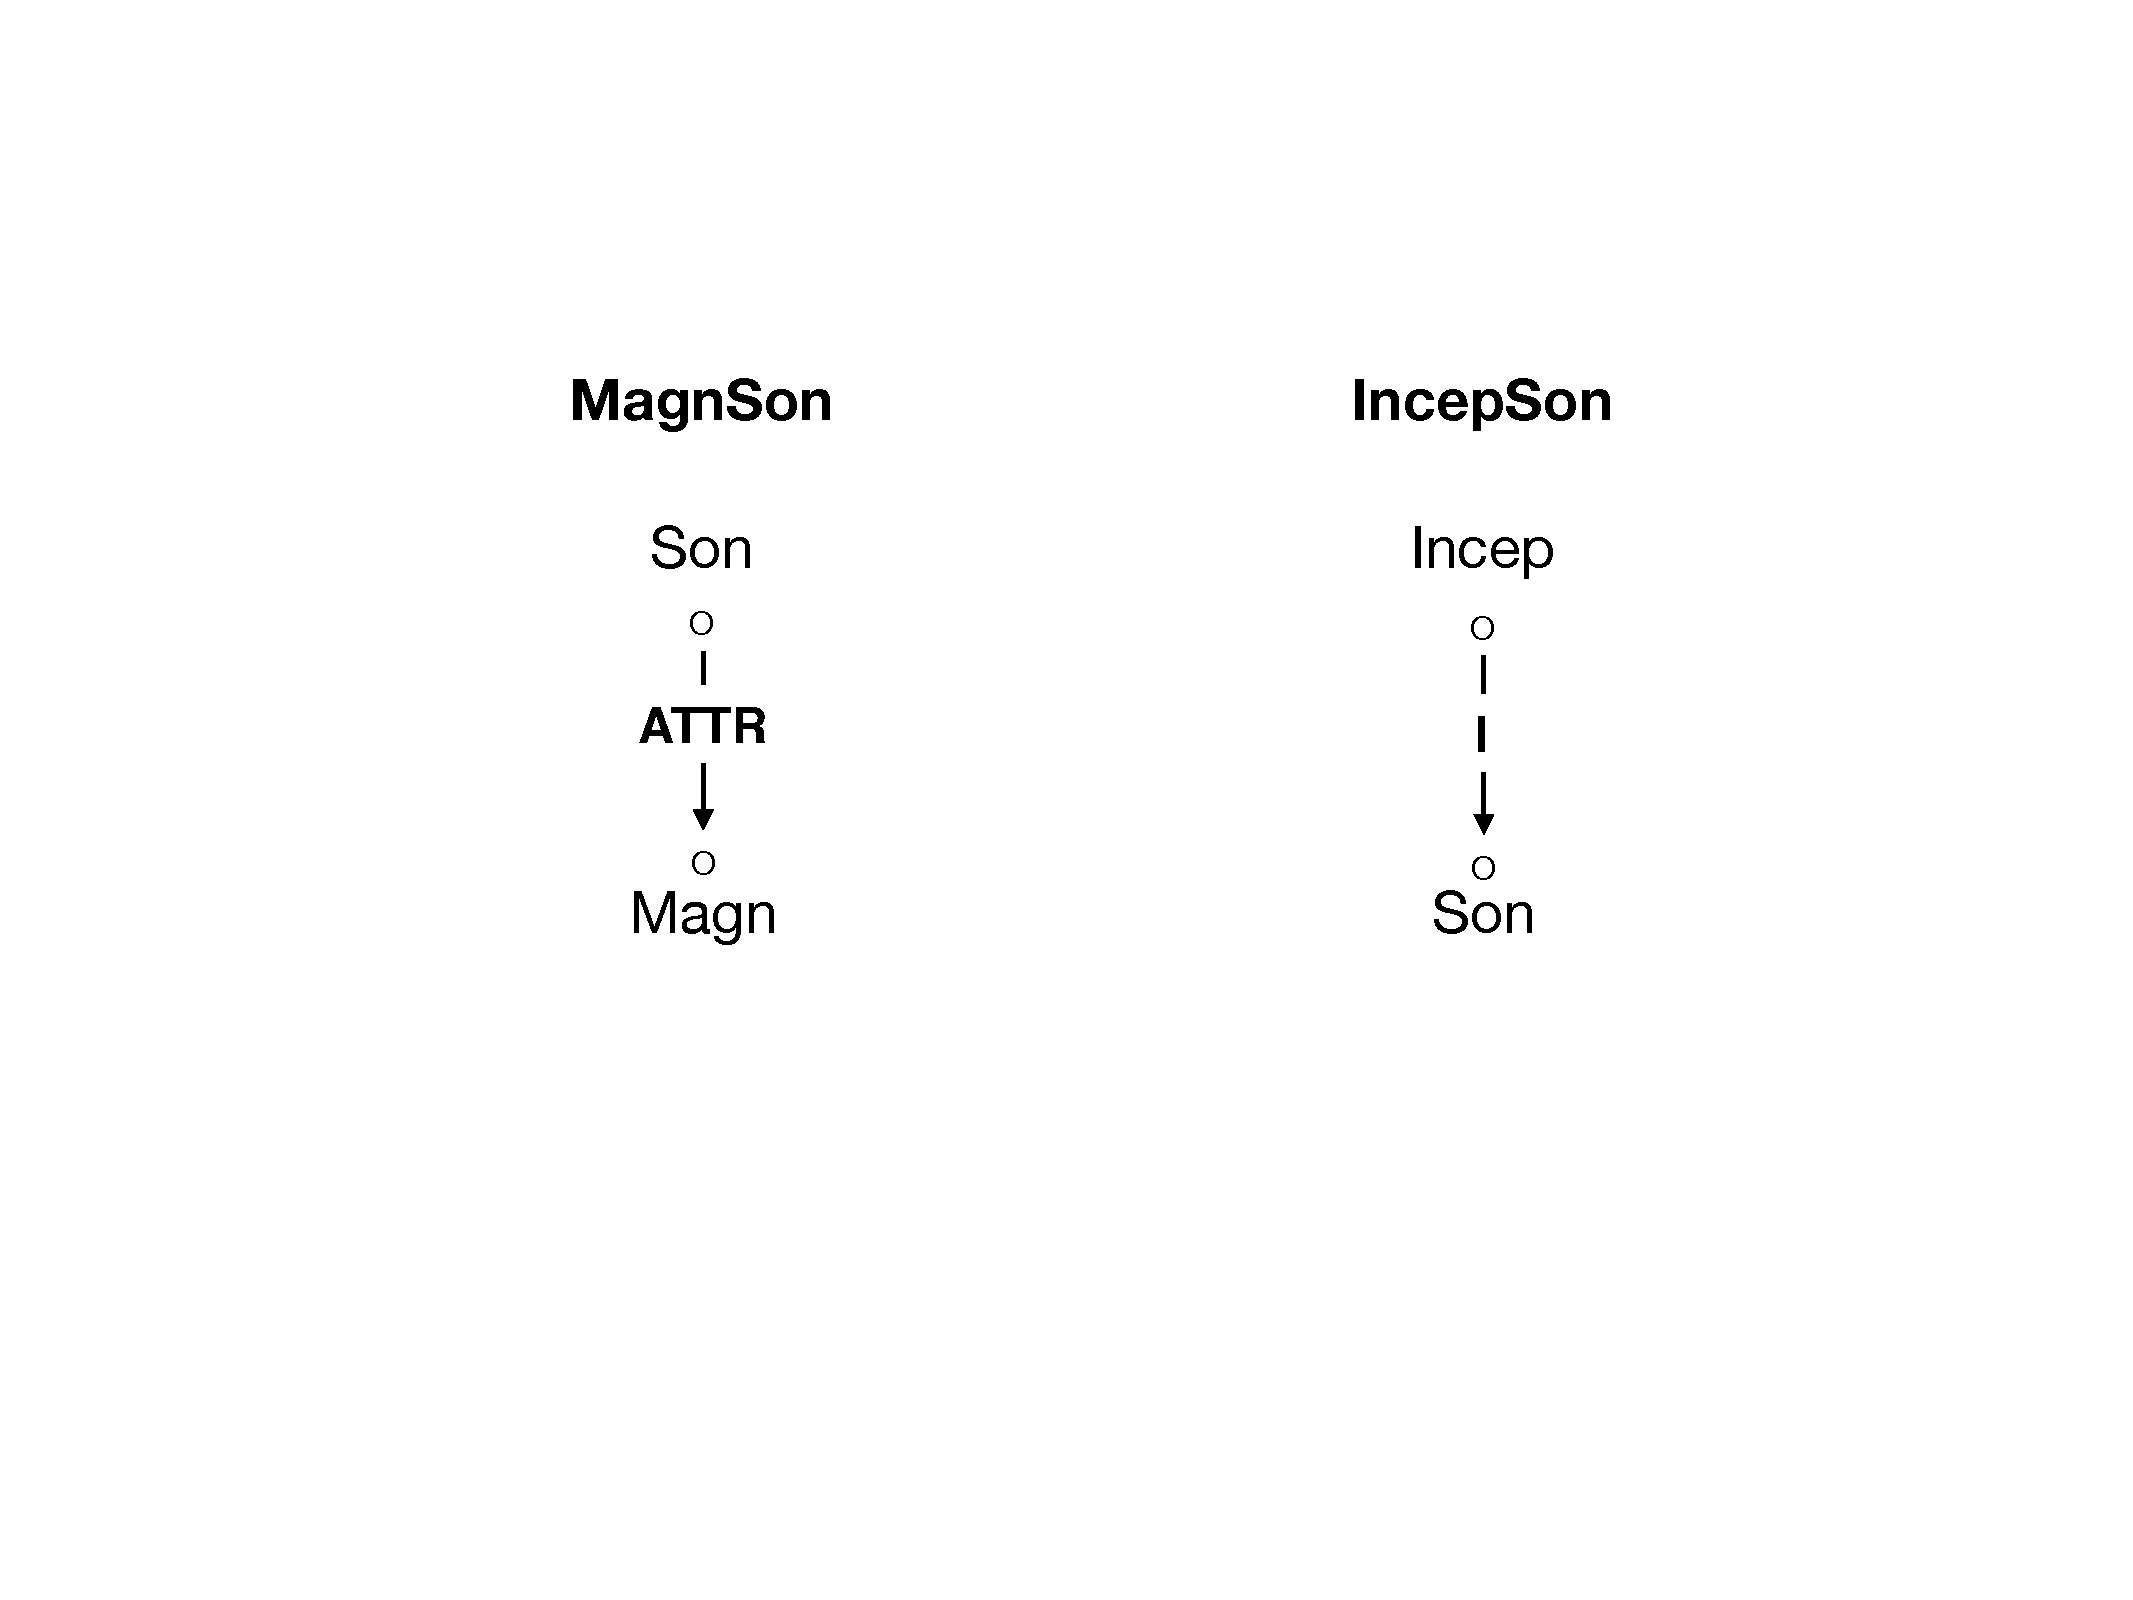
\includegraphics[width=5.3cm]{Fig/NotionLF/ComplexLFDSyntStruct.pdf}
\caption{DSyntSs of complex LFs \lf{MagnSon} and \lf{IncepSon}}\label{fig:ComplexLFDSyntStruct}
\end{figure}

\phantomsection\label{par:PoSComplexLF}\begin{soundbox}{Part of speech of a complex LF}
The head [=~top node] of the DSyntS of a complex LF gives its part of speech\index[notion]{complex LF!part of speech of a \tld}\index[notion]{lexical function!part of speech of a \tld}\index[notion]{part of speech [PoS]!\tld\ of an LF} to the value elements of this LF. For instance, the value of \lf{S\tsub{loc}Real\tsub{1}} -- whose DSyntS is \lf{S\tsub{loc}}\thinspace\syntRel{II}\thinspace\lf{Real\tsub{1}} -- is a noun (as \lf{S\tsub{loc}}), and the value of \lf{MagnSon} -- whose DSyntS is \lf{Magn}\thinspace\syntRelLeft{ATTR}\thinspace\lf{Son} -- is a verb (as \lf{Son}).

The part of speech of simple standard LFs is presented in detail in \sectref{sec:PofS} (p.\thinspace\pageref{sec:PofS}).

\end{soundbox}

A complex LF can consist of more than two simple LFs. For instance, \figref{fig:ComplexComplexLFDSyntStruct} shows the DSyntSs of such complex LFs exemplified in \Next:

\begingroup
\small

\ex. \a. \begingroup\setlength{\tabcolsep}{2pt}
\begin{tabular}[t]{ l l >{\raggedright\arraybackslash}p{7cm} }
\lfappl{AntiBonReal\tsub{1}}{\textit{chair}\tsub{(N)}} & = & \textit{slouch}\tsub{(V)}\textbf{,} \textit{slump}\tsub{(V)} \lfgp{\textit{in} \textsc{art} \tld} \\*
%\lfappl{A\tsub{1}AntiBonReal\tsub{1}}{\textit{chair}\tsub{(N)}} & = & \textit{slouched}\textbf{,} \textit{slumped} \lfgp{\textit{in} \textbf{\textsc{art}} \tld}\\
\end{tabular}\endgroup
    \b. \begingroup\setlength{\tabcolsep}{2pt}
\begin{tabular}[t]{ l l >{\raggedright\arraybackslash}p{6cm} }
\lfappl{CausPlusFact\tsub{0}}{\textit{screw}\tsub{(N)}} & = & \textit{tighten} \lfgp{\textsc{art}}\\[2pt]
\multicolumn{3}{>{\raggedright\arraybackslash}p{10cm}}{\remark{Note.}\lf{CausPlusFact\tsub{0}} is an abbreviation of \lf{CausPlusMagnFact\tsub{0}} -- see \chapref{chap:syntLFs}, [\ref{lf:Plus}], ``\nameref*{par:PlusMagn},'' p.\thinspace\pageref{par:PlusMagn}.} \\
\end{tabular}\endgroup

\endgroup

\begin{figure}

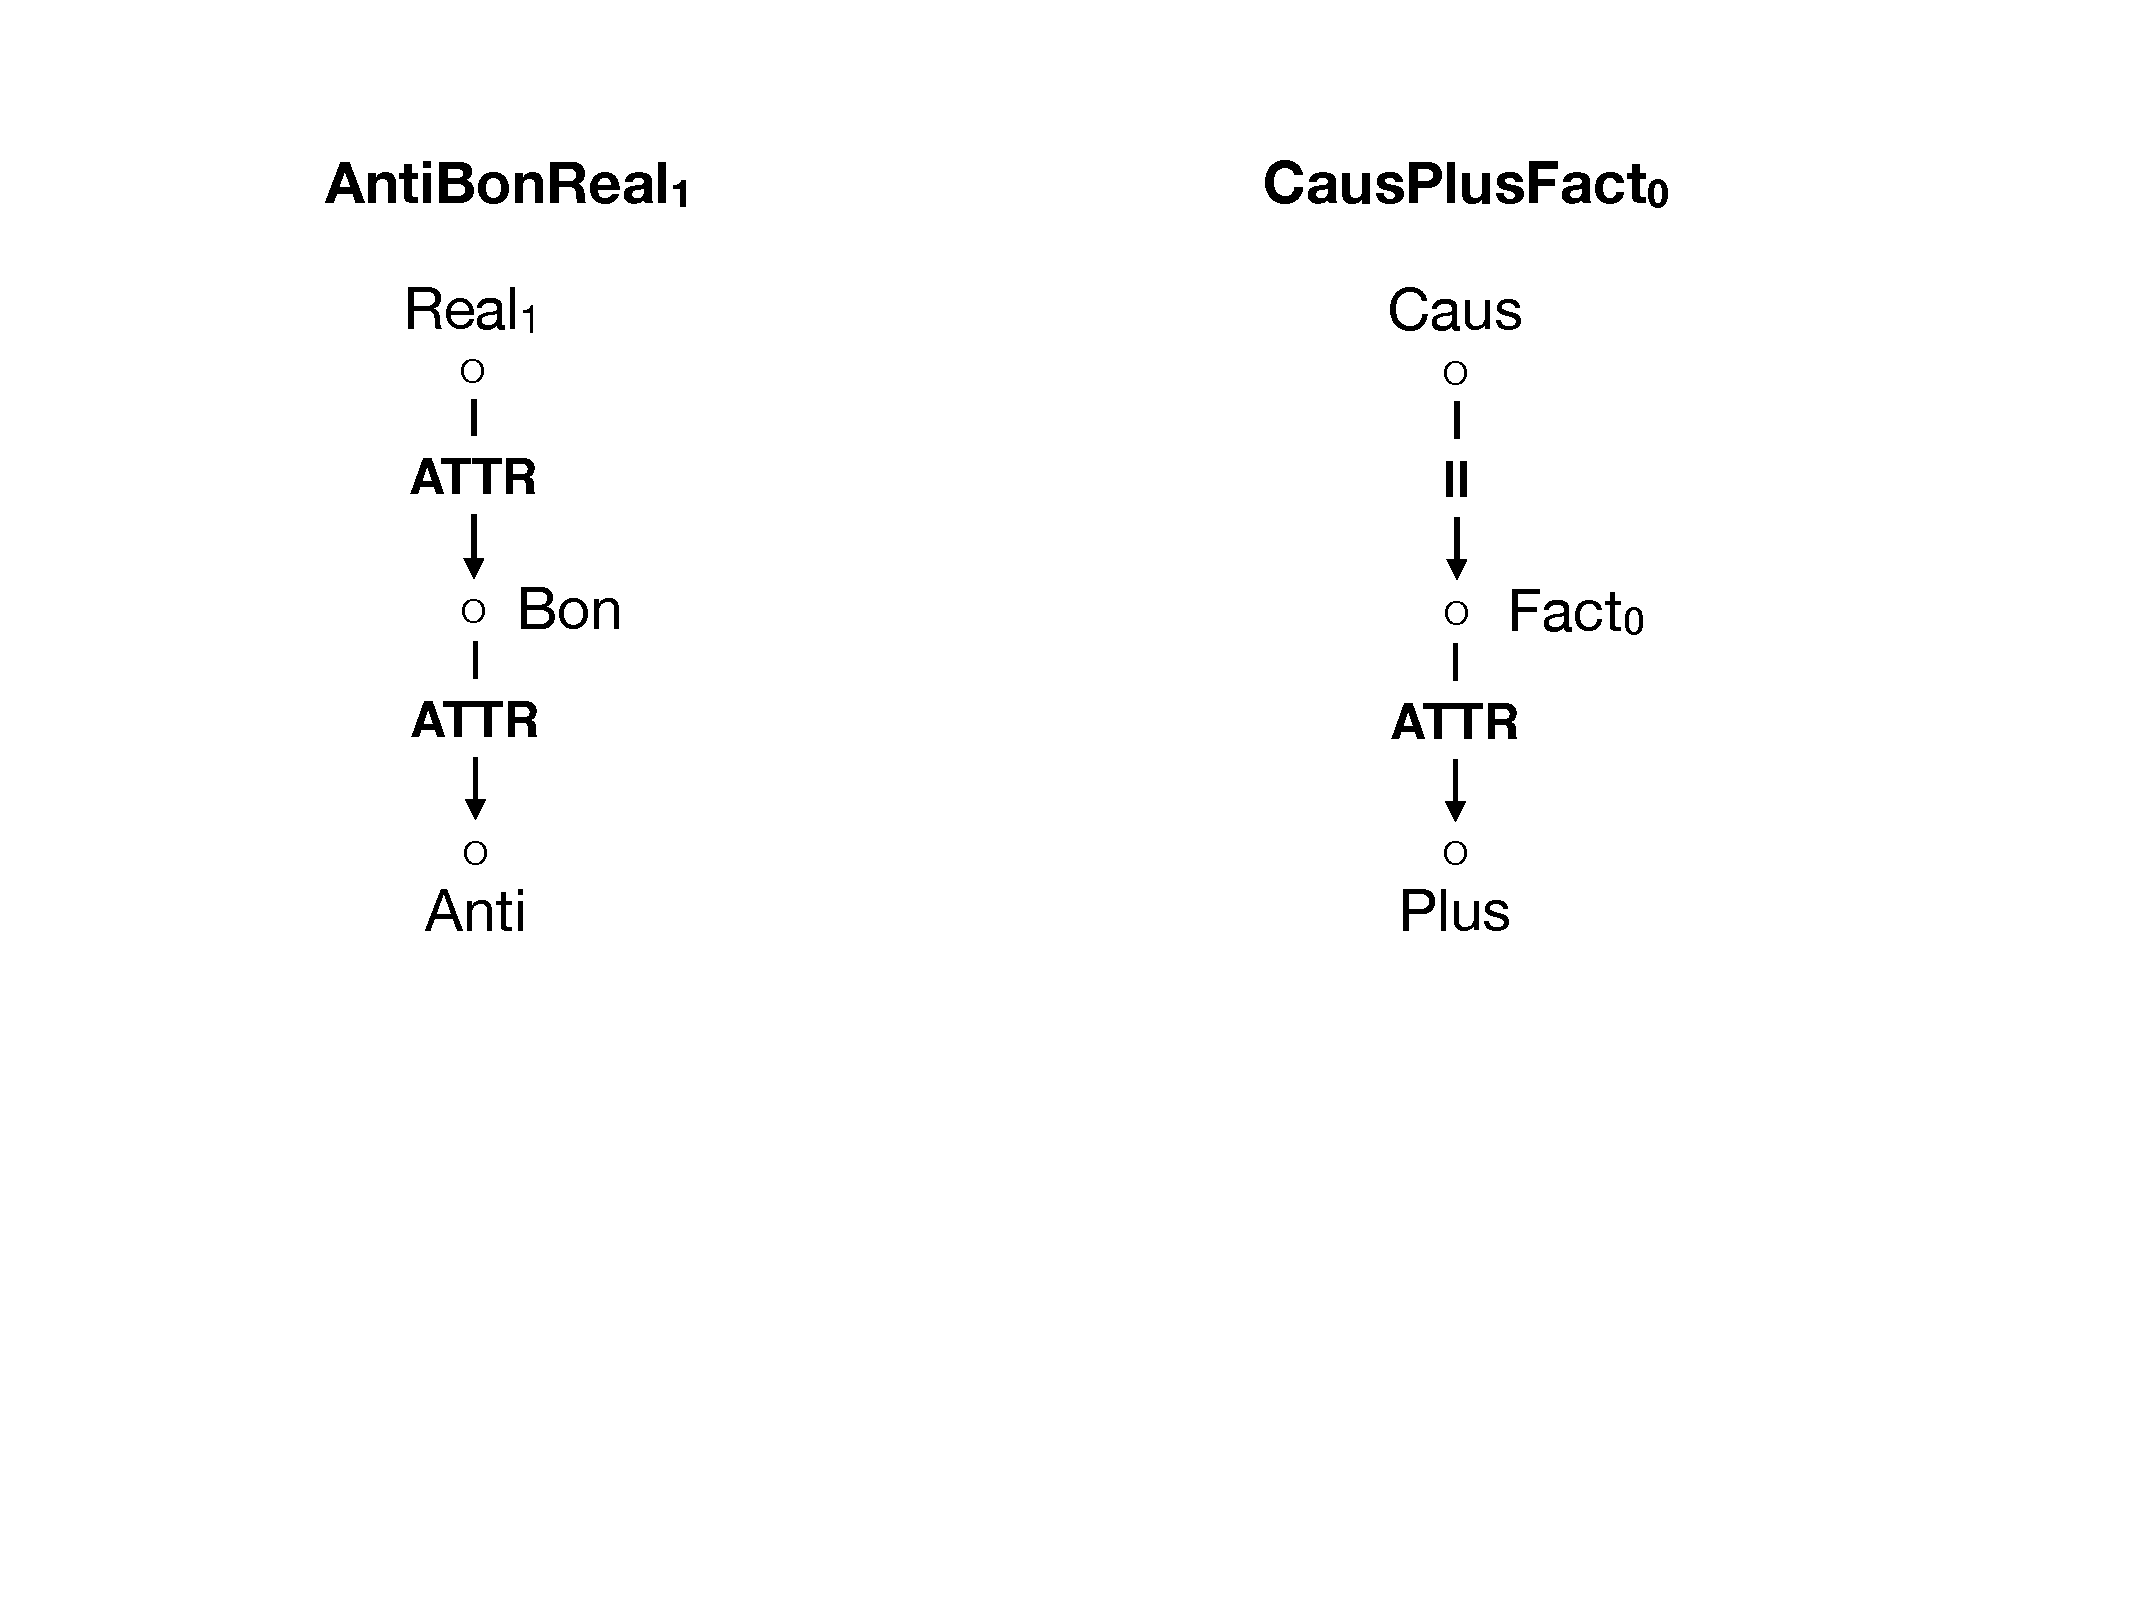
\includegraphics[width=6.7cm]{Fig/NotionLF/ComplexComplexLFDSyntStruct.pdf}
\caption{DSyntSs of complex LFs \lf{AntiBonReal\tsub{1}} and \lf{CausPlusFact\tsub{0}}}\label{fig:ComplexComplexLFDSyntStruct}
\end{figure}

\subsection{Configurational LFs}\label{sec:FLConfigurationnelles}\index[notion]{lexical function!configurational \tld|emph}\index[notion]{configurational LF|emph}

The combination of two LFs \lf{f\tsub{1}} and \lf{f\tsub{2}} can be such that both LFs apply to L simultaneously, but independently of each other and return a single value expressing jointly both LFs. This is represented by the following formula: \lfappl{f\tsub{1}+f\tsub{2}}{L}.

An \lf{f\tsub{1}+f\tsub{2}} configuration is called a \notion{configurational LF}. Compare the following pair of LFs:

\begingroup
\small

\ex. \begingroup\setlength{\tabcolsep}{2pt}
\begin{tabular}[t]{ l l >{\raggedright\arraybackslash}p{3cm} l }
\lfappl{A\tsub{1}}{\textit{sweat}\tsub{(V)}} & = & \textit{sweaty} & `who is sweating' \\*
\lfappl{Magn+A\tsub{1}}{\textit{sweat}\tsub{(V)}} & = & \textit{drenched in sweat}\tsub{(N)} & `who is sweating a lot'\vspace{3pt} \\
%\lfappl{A\tsub{1}}{\textit{despair}\tsub{(N)}} & = & \textit{in} \tld \\
%\lfappl{Magn\thinspace+\thinspace A\tsub{1}}{\textit{despair}\tsub{(N)}} & = & \idiom{\textit{in the pit}} \textit{of} \tld \\
\end{tabular}\endgroup

\endgroup\index[lf]{Magn@\lf{Magn}}\index[lf]{Ai@\lf{A\tsub{i}}!\lf{A\tsub{1}}}

\phantomsection\label{para:orderComponents}In a configurational LF \lf{f\tsub{1}+f\tsub{2}}, the order of components is relevant: \lf{f\tsub{2}} -- the rightmost LF -- is dominant, both syntactically and informationally. In the configuration \lf{f\tsub{1}+f\tsub{2}} where \lf{f\tsub{1}} and \lf{f\tsub{2}} are of different parts of speech\index[notion]{part of speech [PoS]!\tld\ of an LF}\index[notion]{lexical function!part of speech of a \tld}\index[notion]{configurational LF!part of speech of a \tld}, the component \lf{f\tsub{2}} imposes its part of speech on the value of the configurational LF, i.e., it dominates \lf{f\tsub{1}} syntactically. For instance, in the example below, the value is a verb, in accordance to the \lf{Oper\tsub{1}} component of the configurational LF:

\begingroup
\small

\ex. \begingroup\setlength{\tabcolsep}{2pt}
\begin{tabular}[t]{ l l >{\raggedright\arraybackslash}p{7cm} }
\lfappl{Magn+Oper\tsub{1}}{\textit{desire}\tsub{(N)}} & = & \textit{simmer} \lfgp{\textit{with} \tld} \\
\end{tabular}\endgroup

\endgroup\index[lf]{Magn@\lf{Magn}}\index[lf]{Operi@\lf{Oper\tsub{i}}!\lf{Oper\tsub{1}}}

If \lf{f\tsub{1}} and \lf{f\tsub{2}} are of the same part of speech -- e.g., both are modifying adjectives -- the meaning of \lf{f\tsub{2}} constitutes the informationally dominant component in the meaning of the value. For instance, the contrast between \lf{Bon+Magn} and \lf{Magn+Bon} is illustrated in \Next:

\begingroup
\small

\ex. \begingroup\setlength{\tabcolsep}{2pt}
\begin{tabular}[t]{ l l >{\raggedright\arraybackslash}p{2cm} l }
\lfappl{Bon+Magn}{\textit{meal}} & = & \textit{hearty} & `copious, and also good' \\*
\lfappl{Magn+Bon}{\textit{meal}} & = & \textit{somptuous} & `good, and also copious' \\
\end{tabular}\endgroup

\endgroup\index[lf]{Magn@\lf{Magn}}\index[lf]{Bon@\lf{Bon}}

\subsection{Actantial subscripts in LF combinations}\label{sec:actSubsLFCombinations}

\subsubsection{Actantial subscripts in complex LFs}

Two cases are to be distinguished for the actantial subscript to the name of a simple LF \lf{f\tsub{i}} used as a component of a complex LF (except for the rightmost one in the formula, which is interpretable in the standard way).

If \lf{f\tsub{i}} in a complex formula \lf{f\tsub{i}g} is not a verb of causing (\chapref{chap:syntLFs}, \sectref{sec:collocCausatif}\index[notion]{verb!\tld\ of causing}), its argument is the next simple LF \lf{g}, and  its actantial subscript ``\tsub{\lf{i}}'' refers to the DSyntA\thinspace\syntDname{i} of \lf{g}. For instance, in the complex LF \lf{A\tsub{1}Real\tsub{2}}\index[lf]{Ai@\lf{A\tsub{i}}!\lf{A\tsub{1}}}\index[lf]{Reali@\lf{Real\tsub{i}}!\lf{Real\tsub{2}}}, illustrated in \Next, ``\tsub{\lf{1}}'' refers to the DSyntA\thinspace\syntDname{I} of \lf{Real\tsub{2}} -- that is, to the sick person taking the medication.

\begingroup
\small

\ex. \lfappl{A\tsub{1}Real\tsub{2}}{\textit{medication} \lfgp{\textit{prescribed by X to Y against Z}}} = \textit{medicated}\textbf{,} \textit{on} \tld

\endgroup

The actantial subscripts of the LF \lf{A\tsub{1}Real\tsub{2}} used in \Last are interpretable as follows:

\begin{itemize}

\item The lexical unit \textsc{medication} controls three DSyntAs: DSyntA\thinspace\sensenum{I} is the doctor X; DSyntA\thinspace\sensenum{II}, the sick person Y; DSyntA\thinspace\sensenum{III}, the illness Z.

\item \lfappl{Real\tsub{2}}{\textit{medication}} -- \lfgp{\textit{Y}} \textit{takes} \lfgp{\textit{a medication}} -- controls, by definition of the LF \lf{Real\tsub{i}} (\chapref{chap:syntLFs}, [\ref{lf:Real-i}], p.\thinspace\pageref{lf:Real-i}), two DSyntAs:

\begin{itemize}

\item DSyntA\thinspace\syntDname{I}, the sick person Y -- cf. ``\tsub{\lf{2}}'' in \lf{Real\tsub{\textbf{2}}} (since Y is DSyntA~\syntDname{II} of \textsc{medication});
 
 \item DSyntA\thinspace\syntDname{II}, the noun \textsc{medication}.

\end{itemize}

\item The subscript ``\tsub{\lf{1}}'' of \lf{A\tsub{1}} in the formula \lf{A\tsub{1}Real\tsub{2}} refers to the DSyntA\thinspace\syntDname{I} of its argument \lf{Real\tsub{2}}, that is, to the sick person Y (and not to the DSyntA\thinspace\sensenum{I} of \textsc{medication}, that is, to the doctor~X).

\end{itemize}

If \lf{f\tsub{i}} is  a verb of causing, its actantial subscript\index[notion]{actantial subscript!\tld\ of a verb of causing LF} ``\tsub{i}'' refers to the corresponding DSyntA of L, just as it does when this LF is used alone. For instance, in the complex LF \lf{Caus\tsub{2}Oper\tsub{2}}\index[lf]{Caus@\lf{Caus}!\lf{Caus\tsub{2}}}\index[lf]{Operi@\lf{Oper\tsub{i}}!\lf{Oper\tsub{2}}} illustrated in \Next, the subscript ``\tsub{\lf{2}}'' of \lf{Caus\tsub{2}} refers to the DSyntA\thinspace\syntDname{II} of \textit{trust}\tsub{(N)}, that is, to the person who is trusted:

\begingroup
\small

\ex. \lfappl{Caus\tsub{2}Oper\tsub{2}}{\textit{trust}\tsub{(N)} \lfgp{\textit{of X in Y}}} = \textit{win}\tsub{(V)} \lfgp{\textsc{art} \tld} \\
     Ex.: \textit{Joey}\tsub{Y} \textit{won}\tsub{\lfappl{Caus$_\text{2}$Oper$_\text{2}$}{\textit{trust}\tsub{(N)}}} \textit{the trust of Chandler}\tsub{X}\textit{.}

\endgroup

\subsubsection{Actantial subscripts in configurational LFs}

There is nothing  particular to be said about actantial subscripts\index[notion]{actantial subscript} in configurational LFs: the components of these LFs are either simple LFs, or complex LFs, and the explanations about actantial subscripts in these two types of LFs have already been provided.

\section{Parts of speech of simple standard LFs}\label{sec:PofS}

Since an LF is a deep lexical unit\index[notion]{lexical unit!deep \tld} (cf.~\ref{sec:LFAsDeepLU}, p.\thinspace\pageref{sec:LFAsDeepLU}), it belongs to a part of speech\index[notion]{lexical function!part of speech of a \tld}\index[notion]{part of speech [PoS]!\tld\ of an LF}. More specifically, as we will see, it has only a deep-syntactic part of speech.

\subsection{Notion of part of speech [PoS]}\label{sec:notionPdD}

A \notion{part of speech}\index[notion]{part of speech [PoS]|emph} [\notion{PoS}\index[notion]{PoS|see{part of speech}}] is a major class of lexical units that feature, at the syntactic level, the same \notion{passive syntactic valence}\index[notion]{valence!passive syntactic \tld|emph}. By passive syntactic valence of a lexical unit, we mean its ability to participate in particular syntactic constructions as the dependent\index[notion]{dependent, syntactic} member \parencite[109]{Melcuk2015a-e}:\footnote{Passive syntactic valence is to be contrasted with active syntactic valence, introduced in \chapref{chap:preliminaryNotions}, \sectref{sec:syntacticNotions}, p.\thinspace\pageref{para:activeSyntacticValence}.}\index[notion]{valence!active syntactic \tld}

\begin{itemize}

\item a verb -- in a finite form -- is typically the syntactic head of a clause and need not be dependent;
\item a noun is typically a syntactic actant;
\item an adjective is typically a modifier of a noun;
\item etc.

\end{itemize}

Two types of PoS are distinguished: deep PoS and surface PoS. There are five \notion{deep parts of speech}\index[notion]{part of speech [PoS]!deep \tld|emph}:

\begin{itemize}

\item \notion{Verb} [\notion{V}]\index[notion]{verb!Verb [V]|emph}\index[notion]{part of speech [PoS]!V(erb)|emph},
\item \notion{Noun} [\notion{N}]\index[notion]{noun!Noun [N]|emph}\index[notion]{part of speech [PoS]!N(oun)|emph},
\item \notion{Adjective} [\notion{Adj}]\index[notion]{adjective!Adjective [Adj]|emph}\index[notion]{part of speech [PoS]!Adj(ective)|emph},
\item \notion{Adverb} [\notion{Adv}]\index[notion]{adverb!Adverb [Adv]|emph}\index[notion]{part of speech [PoS]!Adv(erb)|emph},
\item \notion{Clausative} [\notion{Claus}]\index[notion]{clausative!Clausative [Claus]|emph}\index[notion]{part of speech [PoS]!Claus(ative)|emph}.

\end{itemize}

V, N, Adj and Adv do not call for further remarks. Claus, on the other hand, needs an explanation: a clausative is a lexical expression that is syntactically equivalent to an independent clause and is not a verb.\footnote{\textcite[Ch.~45]{Tesniere1959} calls such expressions \textit{mots phrases} or \textit{phrasillons}.} \phantomsection\label{txt:Claus0}Clausatives form a very heterogenous lexical class, which includes emotional interjections\index[notion]{interjection} (\textsc{Wow!}, \textsc{Yuck!}) and onomatopoeic interjections\index[notion]{onomatopoeia}\index[notion]{interjection!onomatopoeic \tld} (\textsc{Meow!}, \textsc{Bang!}), as well as interjection-like lexemes (\textsc{Well}) and fixed phrases (\idiom{\textsc{Bless you}} \lfgp{to someone who just sneezed}\footnote{Even if \textsc{bless} is inherently a verb, the phrase \textit{Bless you!} is not a verbal phrase: the form \textit{bless} in it obviously cannot be considered an imperative, and neither can it be taken to be a finite form, since it has no subject. This form is ``frozen'' not only semantically, but also syntactically.}).

Deep PoS are linguistically universal\index[notion]{language-universal} in the sense that they are necessary and sufficient for describing deep-syntactic structures\index[notion]{structure!deep-syntactic \tld\ [DSyntS]}\index[notion]{deep-syntactic!\tld\ structure [DSyntS]} of sentences in any language.

In contrast to deep PoS, \notion{surface PoS}\index[notion]{part of speech [PoS]!surface \tld|emph} are not linguistically universal: each language features its own set of surface PoS. Thus, English has prepositions\index[notion]{preposition}, while Hungarian has only postpositions\index[notion]{postposition}; English has determiners\index[notion]{determiner}, while Russian does not. A given surface PoS is a ``particular case'' of a deep PoS: prepositions and conjunctions\index[notion]{conjunction} are subtypes of deep adverbs (Adv)\index[notion]{adverb};\footnote{More precisely, prepositions and conjunctions form a subclass of adverbs that have an obligatory DSyntA\thinspace\syntDname{II} (on DSyntA, see \chapref{chap:preliminaryNotions}, \sectref{sec:syntacticNotions}, p.\thinspace\pageref{def:DSyntA}).}\index[notion]{actant!deep-syntactic \tld\ [DSyntA]}\index[notion]{deep-syntactic!\tld\ actant [DSyntA]} determiners are subtypes of deep adjectives\index[notion]{adjective} (Adj); etc. On deep vs. surface PoS, see \textcite[Ch.~7, Sec.~2.1.3, 49--51]{Melcuk2013c-e}.\phantomsection\label{txt:PrepAdv}

In what follows, only deep PoS are considered, so that the adjective \textit{deep} can be omitted.

To conclude, note that the PoS of a lexical unit L is a core element of L's cooccurrence\index[notion]{cooccurrence, restricted}; as such, it can be expected to be the first piece of information given in L's lexical entry\index[notion]{lexical entry}\index[notion]{lexicography} -- see e.g., the lexical entry of \textsc{anger}\tsub{(N)} in the Appendix (p.\thinspace\pageref{chap:appendix1}).

\subsection{LF's inherent PoS}\label{sec:LFsInherentPoS}

Most simple standard LFs possess an inherent PoS\index[notion]{part of speech [PoS]!\tld\ of an LF}\index[notion]{lexical function!part of speech of a \tld}: e.g., \lfappl{S\tsub{i}}{L}\index[lf]{Si@\lf{S\tsub{i}}} is always a noun, and \lfappl{Oper\tsub{i}}{L}\index[lf]{Operi@\lf{Oper\tsub{i}}} is always a verb. However, several paradigmatic LFs borrow their PoS from their argument. Such LFs are:

\begin{itemize}

\item the three ``meta''-LFs, which underlie the whole LF system\index[notion]{lexical function!system of standard \tlds}\index[notion]{system of standard LFs}: \lf{Syn}\index[lf]{Syn@\lf{Syn}}, \lf{Conv\tsub{ijk}}\index[lf]{Convijk@\lf{Conv\tsub{ijk}}} and \lf{Anti}\index[lf]{Anti@\lf{Anti}} (with \lf{Contr}\index[lf]{Contr@\lf{Contr}}) -- \chapref{chap:paraLFs}, \sectref{sec:troisPiliersFL}, p.\thinspace\pageref{sec:troisPiliersFL};

\item the ``semantic pronoun'': \lf{Gener}\index[lf]{Gener@\lf{Gener}} -- \chapref{chap:paraLFs}, [\ref{lf:Gener}], p.\thinspace\pageref{lf:Gener};

\item two LFs whose meanings are close to those of grammemes\index[notion]{grammeme}: the singulative \lf{Sing}\index[lf]{Sing@\lf{Sing}} and the collective \lf{Mult}\index[lf]{Mult@\lf{Mult}} -- \chapref{chap:paraLFs}, \sectref{sec:flFlexion}, p.\thinspace\pageref{sec:flFlexion}.

\end{itemize}

For the PoS of complex LFs\index[notion]{lexical function!complex \tld}\index[notion]{complex LF}, see \sectref{sec:FLComplexes}, p.\thinspace\pageref{par:PoSComplexLF}.

\paragraph*{Part of speech tables for LF applications.}\label{par:LFPoSTable}\index[notion]{application of an LF!part of speech of the \tld}

An LF \lf{f} calls for two syntactic characteristics as regards PoS: (i)~the PoS of its possible arguments L and (ii)~the corresponding PoS of its value -- a deep lexical unit\index[notion]{lexical unit!deep \tld} \lfappl{f}{L}.

This correspondence is shown in a \notion{PoS table}\index[notion]{part of speech [PoS]!\tld\ table|emph} for each LF. Take as example the PoS table of \lf{Magn}\index[lf]{Magn@\lf{Magn}}, intensification modifier:

\begin{quote}
\small
\begin{tabular}{ l c c c c c }
   \midrule
   \multicolumn{6}{l}{\lf{Magn}: adjectival\slashs{}adverbial} \\
   \midrule
   \textbf{L} & V & N & Adj & Adv & Claus \\
%   \midrule
   \textbf{\lfappl{Magn}{L}} & Adv & Adj & Adv & Adv & Adj\slashs{}Adv \\
   \midrule
\end{tabular}
\end{quote}

The table header indicates that \lf{Magn} is a modifier that functions as an adjective\index[notion]{adjective} or an adverb\index[notion]{adverb}. The body of the table specifies the correspondence between the PoS of L and that of the deep lexical unit \lfappl{Magn}{L} -- i.e., the PoS of \lf{Magn} itself, for short.

When a PoS correspondence is theoretically possible, but not attested to our knowledge, the symbol ``\lfgp{?}'' is added. The PoS table of \lf{Gener}\index[lf]{Gener@\lf{Gener}} illustrates this situation.

\begin{quote}
\small
\begin{tabular}{ l c c c c c }
   \midrule
   \multicolumn{6}{l}{\lf{Gener}: borrows L's PoS} \\
   \midrule
   \textbf{L} & V & N & Adj & Adv & Claus \\
   \midrule
   \textbf{\lfappl{Gener}{L}} & V & N & Adj & Adv & Claus\lfgp{?} \\
   \midrule
\end{tabular}
\end{quote} 

In the header of this table, the statement ``borrows L's PoS'' indicates that \lf{Gener} is an LF without inherent PoS\index[notion]{part of speech [PoS]!inherent \tld}.

\section{Regularities in standard LFs}\label{sec:regularitiesInLFs}

In spite of the basically idiosyncratic character of LFs, in many cases a given LF has the same values for quite a few different arguments: you \textit{take a bath}, \textit{a shower}, \textit{a rest}, ...; you \textit{are in despair}, \textit{love}, \textit{a rage}, ...; you \textit{follow the rules}, \textit{prescriptions}, \textit{recommendations}, \textit{instructions}, ... The reason is, of course, semantic proximity of these LF's arguments: semantically related lexical units tend to feature the same values for a given LF.

In other words, there exist \notion{regularities}\index[notion]{regularity|emph} among LFs of any natural language. No doubt that such regularities play an important role in the acquisition of LFs by speakers, as the former allow the latter to make predictions about LFs. These regularities should be exploited in such domains as language teaching\index[notion]{teaching\slashs{}learning, language}\index[notion]{language teaching\slashs{}learning}, translation, etc. It is therefore important to extract them, and formulate \notion{generalizations}\index[notion]{generalization concerning LFs|emph}, which should be stored in models of the lexicon\index[notion]{lexicon!\tld\ model}\index[notion]{model!lexicon \tld} in a way that supports the \notion{inheritance}\index[notion]{inheritance!\tld\ of regularities}\index[notion]{regularity!inheritance of \tld{ies}} of regularities \parencite{MelcukWanner1996}.

The elements of the values of an LF \lf{f} shared by several argument lexical units can be generalized by extracting them from individual lexical entries\index[notion]{lexical entry} of these units and storing them together: either on the argument side (for a group of lexical units) or on the LF side (attaching them to the LF itself). In practice, both methods can be  combined in different proportions. We propose below four types of generalizations, that is, we indicate types of regularities with associated means of accounting for them: generalizations at vocable's level (\sectref{sec:generalizationVocable}), generalizations associated with a generic term (\sectref{sec:generalizationsGener}), joker values\index[notion]{value of an LF!joker \tld}\index[notion]{joker value of an LF}\index[notion]{lexical function!joker value of a \tld} associated with given LFs (\sectref{sec:jokerValuesAssociatedGivenLFs}) and lexical entries for collocative lexical units (\sectref{sec:lexicalEntriesCollocativesLUs}).

\subsection{Generalizations at vocable's level}\label{sec:generalizationVocable}\index[notion]{generalization concerning LFs!\tld\ associated with a vocable}\index[notion]{vocable}

If several lexical units of a given vocable or of several semantically-related vocables share LF values, these values can be given under one of these units, with a cross-reference in the lexical entries\index[notion]{lexical entry} of the others. For instance, we have for the verb \textsc{escape}{\tsub{(V)}}:

\begingroup
\small

\ex. \begingroup\setlength{\tabcolsep}{2pt}
\begin{tabular}[t]{ l l >{\raggedright\arraybackslash}p{7cm} }
\lf{S\tsub{1}} & : & \textit{escaper} \\
\lf{S\tsub{1}Perf} & : & \textit{escapee}\textbf{,} \textit{fugitive}\tsub{(N)}\textbf{,} \textit{runaway}\tsub{(N)} \\
\lf{S\tsub{1}Able\tsub{1}} & : & \idiom{\textit{flight risk}} \\
%\lf{S$_\text{1}^\text{usual}$} & : & ... \\
\lf{S\tsub{2}} & : & \idiom{\textit{place of detention}} \\
\lf{A\tsub{1}} & : & \textit{fugitive}\tsub{(Adj)}\textbf{,} \textit{runaway}\tsub{(Adj)} \\*
\lf{Able\tsub{2}} & : & \textit{escapable} \\
\end{tabular}\endgroup

\endgroup\index[lf]{Si@\lf{S\tsub{i}}!\lf{S\tsub{1}}}\index[lf]{Perf@\lf{Perf}}\index[lf]{Ablei@\lf{Able\tsub{i}}!\lf{Able\tsub{1}}}\index[lf]{Ablei@\lf{Able\tsub{i}}!\lf{Able\tsub{2}}}\index[lf]{Si@\lf{S\tsub{i}}!\lf{S\tsub{2}}}\index[lf]{Ai@\lf{A\tsub{i}}!\lf{A\tsub{1}}}

As the same LF relations hold for the corresponding noun \textsc{escape}\tsub{(N)}, which is the \lf{S\tsub{0}}\index[lf]{S0@\lf{S\tsub{0}}} (nominalization) of the verb, we can simply indicate the following cross-reference in its lexical entry\index[notion]{lexical entry}:

\begingroup
\small

\ex. \begingroup\setlength{\tabcolsep}{2pt}
\begin{tabular}[t]{ l l >{\raggedright\arraybackslash}p{6cm} }
\lf{S\tsub{1}}\textbf{,} \lf{S\tsub{1}Perf}\textbf{,} \lf{S\tsub{1}Able\tsub{1}}\textbf{,} \lf{S\tsub{2}}\textbf{,} \lf{A\tsub{1}}\textbf{,} \lf{Able\tsub{2}} & : & $\pmb{\uparrow}$\thinspace\textsc{escape}\tsub{(V)} \\
\end{tabular}\endgroup

\endgroup

Note that \Last, which concerns two specific lexical units (\textsc{escape}\tsub{(V)} and \textsc{escape}\tsub{(N)}), is in point of fact a consequence of a series of more general statements concerning the entire system of LFs itself, namely:

\begingroup
\small

\ex. \begingroup\setlength{\tabcolsep}{2pt}
\begin{tabular}[t]{ l c >{\raggedright\arraybackslash}p{7cm} }
\lfappl{S\tsub{i}}{L\tsub{(V)}} & = & \lfappl{S\tsub{i}}{\lfappl{S\tsub{0}}{L\tsub{(V)}}} \\*
... & & \\
\lfappl{A\tsub{i}}{L\tsub{(V)}} & = & \lfappl{A\tsub{i}}{\lfappl{S\tsub{0}}{L\tsub{(V)}}} \\*
... & & \\
\end{tabular}\endgroup

\endgroup

\subsection{Generalizations associated with a generic term}\label{sec:generalizationsGener}\index[notion]{generalization concerning LFs!\tld\ associated with a generic term}

There are semantic classes\index[notion]{semantic!\tld\ class} of lexical units such that:

\begin{enumerate}

\item they all belong to the same semantic field\index[notion]{semantic!\tld\ field};

\item they possess the same generic term\index[notion]{generic term}\index[lf]{Gener@\lf{Gener}} L\tsub{\textsc{gener}}\footnote{On generic terms, see the LF \lf{Gener}, \chapref{chap:paraLFs}, [\ref{lf:Gener}], p.\thinspace\pageref{lf:Gener}.} -- for instance, \textsc{car}, \textsc{truck}\tsub{(N)}, \textsc{van}, \textsc{bus}\tsub{(N)}, \textsc{motorbike}\tsub{(N)}, ... form a semantic class united under the same L\tsub{\textsc{gener}} \textsc{vehicle} in the sense of `motor vehicle';

\item the meaning of L\tsub{\textsc{gener}} is sufficiently rich so that it belongs to the same semantic field as these lexical units -- cf., \textsc{vehicle} belongs to the same semantic field as \textsc{car}, \textsc{truck}\tsub{(N)}, etc.

\end{enumerate}

Elements of such semantic classes may share the same values for some LFs. (This is only a tendency, with many exceptions, yet in some cases this tendency is quite clear.) If such is the case, generalizations can be made by storing all common values of LFs supplied with necessary constraints under a special \notion{public zone}\index[notion]{lexical entry!public zone of a \tld|emph}\index[notion]{zone of a lexical entry!public \tld|emph} of L\tsub{\textsc{gener}}'s lexical entry. For instance, if the following is stored in the public zone of the lexical entry for \textsc{vehicle}, it does not need to be repeated in the lexical entry for all names of vehicles:

\begin{center}
\footnotesize
\APolbox{10.8cm}{%
\renewcommand*{\arraystretch}{1}
\setlength{\tabcolsep}{2.5pt}
\begin{tabular}{ l l l }
\multicolumn{3}{l}{\textsc{vehicle}, noun} \\
... & & \\
\multicolumn{3}{l}{\textbf{\textsf{Public}}} \vspace{-3pt}\\
... & & \\
\lf{S\tsub{1}}\index[lf]{Si@\lf{S\tsub{i}}!\lf{S\tsub{1}}} & : & \textit{driver}\textbf{;} \textit{rider} \lfconstr{for two-wheel vehicle} \\
\lf{S\tsub{2}}\index[lf]{Si@\lf{S\tsub{i}}!\lf{S\tsub{2}}} & : & \textit{passenger} \\
... & & \\
\lf{Real\tsub{1}}\index[lf]{Reali@\lf{Real\tsub{i}}!\lf{Real\tsub{1}}} \lfgp{i.e., `use \tld\ as driver'} & : & \textit{drive}\tsub{(V)} \lfgp{\textsc{art} \tld}\textbf{;} \textit{ride}\tsub{(V)}\sensenumonly{1} \lfgp{\textsc{art} \tld} \lfconstr{for two-wheel vehicle} \\
\lf{Real\tsub{2}}\index[lf]{Reali@\lf{Real\tsub{i}}!\lf{Real\tsub{2}}} \lfgp{i.e., `use \tld\ as passenger'} & : & \textit{ride}\tsub{(V)}\sensenumonly{2} \lfgp{(\textit{in}\slashs\textit{on}) \textsc{art} \tld}\textbf{,} \textit{go} \lfgp{\textit{by} \tld} \\
... & & \\
\end{tabular}
}
\end{center}

A rather straightforward particular case of the above type generalization is the use of LFs with proper names\index[notion]{proper name}\index[notion]{noun!proper name \tld}. If the argument of an LF \lf{f} happens to be a proper name N\tsub{(prop)}, the value of \lf{f} must be computed substituting for N\tsub{(prop)} the lexical unit L that denotes the entity named by N\tsub{(prop)}. In other words, the values of LFs for \textsc{Rhine}, \textsc{Ganges}, \textsc{Volga}, \textsc{Thames}, \textsc{Mississippi}, etc. are those of the LFs for \textsc{river} (or \textsc{watercourse}):

\begingroup
\small

\ex. \a. The Rhine $\langle$This river$\rangle$ \emph{flows} from Switzerland to the North Sea.
     \b. The Ganges $\langle$This river$\rangle$ \emph{empties} into the Bay of Bengal.
     \c. The Oka $\langle$This river$\rangle$ is a \emph{tributary} of the Volga.
     \d. The Thames $\langle$This river$\rangle$ was \emph{swollen} and \emph{flooding} the riverbanks.

\endgroup

\subsection{Joker values associated with given LFs}\label{sec:jokerValuesAssociatedGivenLFs}\index[notion]{generalization concerning LFs!\tld\ associated with an LF}\index[notion]{value of an LF!joker \tld|emph}\index[notion]{joker value of an LF|emph}\index[notion]{lexical function!joker value of a \tld|emph}

The level of generality of LF values might be such that it becomes feasible to associate with a given LF some general default elements of its value: we refer to such default elements as \notion{joker values}. Thus, a generally valid expression in English of the LF \lf{S\tsub{0}}\index[lf]{S0@\lf{S\tsub{0}}!joker \tld} for a verb L\tsub{(V)} is the phrase \textit{the fact of V-ing} -- or just simply \textit{V-ing}; e.g.:

\begingroup
\small

\ex. \begin{tabular}[t]{ l l l }
\lfappl{joker S\tsub{0}}{\textit{chew}\tsub{(V)}} & = & \textit{the fact of chewing}\textbf{,} \textit{the chewing} \\
\lfappl{joker S\tsub{0}}{\textit{ponder}} & = & \textit{the fact of pondering}\textbf{,} \textit{the pondering} \\
\end{tabular}

\endgroup

For the support verbs\index[notion]{support verb}\index[notion]{verb!support \tld} \lfappl{Oper\tsub{1}}{L}\index[lf]{Operi@\lf{Oper\tsub{i}}!joker \lf{Oper\tsub{1}}}, the joker value elements are \textsc{do}, \textsc{make}, \textsc{give}, \textsc{have}, \textsc{take}, \idiom{\textsc{carry out}} and maybe some more. Of course, for each of those, semantic restrictions on L have to be specified. For \lfappl{Func\tsub{0}}{L}\index[lf]{Funci@\lf{Func\tsub{i}}!joker \lf{Func\tsub{0}}} -- another type of support verbs, joker value elements are, among others, \idiom{\textsc{take place}}, \textsc{happen} (for L denoting a social event), etc. For intensifiers \lfappl{Magn}{L}\index[lf]{Magn@\lf{Magn}!joker \tld}, when they have nominal arguments, such general elements are: \textsc{big}\tsub{(Adj)}, \textsc{high}\tsub{(Adj)} (for L denoting non-linear physical parameters such as \textsc{pressure}\tsub{(N)}, \textsc{speed}\tsub{(N)}, \textsc{temperature}), \textsc{utmost}\tsub{(Adj)}\slashs\textsc{utter}\tsub{(Adj)} (for feelings), etc. An obvious \lf{Magn} joker value element for adjectival lexemes as arguments is \textsc{very}.

The generalizations considered here are directly associated with LFs and their description presupposes the existence of special lexical entries dedicated to LFs\index[notion]{lexical entry!\tld\ for an LF}.

\subsection{Lexical entries for collocative lexical units}\label{sec:lexicalEntriesCollocativesLUs}\index[notion]{lexical entry}\index[notion]{generalization concerning LFs!\tld\ associated with a collocative lexical unit}

\notion{Collocative lexical units}\index[notion]{lexical unit!collocative \tld|emph} are ``designed'' to be selected by the Speaker as values of syntagmatic LFs\index[notion]{lexical function!syntagmatic \tld}\index[notion]{syntagmatic!\tld\ lexical function}: they have virtually no autonomy and are essentially used as collocates\index[notion]{collocation!collocate of a \tld} within collocations\index[notion]{collocation}.

To ensure a sufficiently systematic description of collocative lexical units shared by many collocation bases\index[notion]{base!\tld\ of a collocation}\index[notion]{collocation!base of a \tld}, one has to compile for them special lexical entries\index[notion]{lexical entry!\tld\ for a collocative lexical unit}, where semantic and syntactic conditions on their use are specified. Thus, the support verb\index[notion]{support verb}\index[notion]{verb!support \tld} \textit{deliver} is an element of the value of the LF \lf{Oper\tsub{1}}\index[lf]{Operi@\lf{Oper\tsub{i}}!\lf{Oper\tsub{1}}} for many nouns of public activities (\textit{deliver a speech}\slashs\textit{a lecture}\slashs\textit{a performance}). It receives a lexical entry of its own in the vocable\index[notion]{vocable} \textsc{deliver}; accordingly, it need not be lexicographically described in all lexical entries for nouns it combines with but can be selected and used following indications found in its own entry.

For an example of a dictionary of collocations\index[notion]{dictionary!\tld\ of collocations}\index[notion]{collocation!dictionary of \tlds} with entries for collocates, see \textcite{Bosque2010}.

To round up the topic, still another perspective of possible generalizations for LFs is opened by accounting for the links between the meaning of a lexical unit L and the LFs applicable to it; for instance:

\begin{itemize}

\item L that is predicative\index[notion]{predicativity} expects actantial paradigmatic derivatives\index[notion]{derivative!semantic \tld}\index[notion]{semantic!\tld\ derivative} -- cf. LFs \lf{S\tsub{i}}\index[lf]{Si@\lf{S\tsub{i}}}, \lf{A\tsub{i}}\index[lf]{Ai@\lf{A\tsub{i}}}, ..., and syntagmatic verbal collocates such as support verbs\index[notion]{support verb}\index[notion]{verb!support \tld} (\lf{Oper\tsub{i}}\index[lf]{Operi@\lf{Oper\tsub{i}}}, ...) and possibly realization verbs\index[notion]{verb!realization \tld}\index[notion]{realization verb} (\lf{Real\tsub{i}}\index[lf]{Reali@\lf{Real\tsub{i}}}, ...).

\item L that denotes an artefact expects realization verbs such as \lf{Real\tsub{1}}\index[lf]{Rea|li@\lf{Real\tsub{i}}!\lf{Real\tsub{1}}}, which expresses `make use of L'.

\item L that denotes something producing sounds expects values for the LF \lf{Son}\index[lf]{Son@\lf{Son}}.

\item L that denotes an inner state of a human expects values for the LFs \lf{Manif}\index[lf]{Manif@\lf{Manif}} (`[L]~manifests itself in (part of the body of) X') and \lf{Sympt\tsub{ijk}}\index[lf]{Symptijk@\lf{Sympt\tsub{ijk}}}.

\item L that denotes a place expects values for the LF \lf{Loc\tsub{in/ad/ab}}\index[lf]{Locin@\lf{Loc\tsub{in}}}\index[lf]{Locad@\lf{Loc\tsub{ad}}}\index[lf]{Locab@\lf{Loc\tsub{ab}}}.

\end{itemize}

The identification and proper modeling of such generalizations is an open research question.

\begin{furtherreading}
On semantic regularities in standard LF applications, see \textcite{Apresjan2009}; on lexical inheritance of LF regularities, see \textcites{MelcukWanner1996}{Barrios2009}; on accounting for regularities in lexical entries for collocates, see \textcite{Reuther1996}; on the lexicographic description of collocates, see \textcite{AlonsoRamosMantha1996,AlonsoRamos2003}; on extracting regularities -- polysemy\index[notion]{polysemy!regular \tld}\index[notion]{regularity!regular polysemy} and lexicographic definitions -- in lexical networks with the LF \lf{Gener}, see \textcite{Polguere2022a}.
\end{furtherreading}\index[notion]{inheritance!\tld\ of regularities}\index[notion]{regularity!inheritance of \tld{ies}}\index[notion]{regularity!extraction of \tld{ies}}\index[notion]{polysemy}\index[notion]{definition!lexicographic \tld}\index[notion]{lexical network}\index[notion]{network \lfgp{see also \textit{graph}}!lexical \tld}\index[lf]{Gener@\lf{Gener}}

\section{Description template for simple standard LFs}\label{sec:descriptionTemplateLF}

In Chapters~\ref{chap:paraLFs} and~\ref{chap:syntLFs}, we follow a three-part template (see below, Parts~A, B and C) for the presentation of each individual LF. This template is illustrated with the LF \lf{S\tsub{0}}\index[lf]{S0@\lf{S\tsub{0}}} (\chapref{chap:paraLFs}, [\ref{lf:S0}], p.\thinspace\pageref{lf:S0}).

\paragraph*{Part A.}

Identification number\index[notion]{lexical function!identification number of a \tld} between square brackets and name of the LF together with its Latin source also between square brackets (cf. the remark on the naming of LFs on p.\thinspace\pageref{txt:LFNames}), followed by a rough characterization.

\begin{quote}

\textbf{{\small [\ref{lf:S0}]} \lf{S\tsub{0}} \lfgp{{\scriptsize Latin} \textit{substantivum}}: nominalization}

\end{quote}

\paragraph*{Part B.}

Semantic-syntactic characterization of the LF, followed by its PoS table\index[notion]{part of speech [PoS]!\tld\ table}.

\begin{quote}
\noindent\lf{S\tsub{0}} applies to a non-nominal lexical unit L and returns a noun having the same meaning as L.

\small
\begin{tabular}{ l c c c c }
   \midrule
   \multicolumn{5}{l}{\lf{S\tsub{0}}: nominal} \\
   \midrule
   \textbf{L} & V & Adj & Adv & Claus \\
   \midrule
   \textbf{\lfappl{S\tsub{0}}{L}} & N & N & N & N \\
   \midrule
\end{tabular}
\end{quote}

If a series of LFs have an identical PoS table, it is extracted and mentioned just once before the presentation of these LFs -- see, e.g., the shared PoS table for \lf{Syn}, \lf{Conv\tsub{ijk}} and \lf{Anti} (\chapref{chap:paraLFs}, \sectref{sec:troisPiliersFL}, p.\thinspace\pageref{tab:PoSTableSynConvAnti}).

\paragraph*{Part C.}

Illustration of the LF in English, French and Russian.

\begin{longtable*}[l]{ p{0.5cm} l l >{\raggedright\arraybackslash}p{7cm} }

& \multicolumn{3}{l}{\textbf{English}} \\*

& \lfappl{S\tsub{0}}{\textit{present}\tsub{(V)}} & = & \textit{presentation}  \\
& \lfappl{S\tsub{0}}{\textit{leave}\tsub{(V)}} & = & \textit{departure}  \\*
& ... & &  \\[6pt]
%& \lfappl{S\tsub{0}}{\textit{fall}\tsub{(V)}} & = & \textit{fall}\tsub{(N)}  \\
%& \lfappl{S\tsub{0}}{\textit{close}\tsub{(Adj)}} & = & \textit{proximity}  \\
%& \lfappl{S\tsub{0}}{\textit{Bang!}} & = & \textit{gunshot}\vspace{6pt}  \\

& \multicolumn{3}{l}{\textbf{French}} \\*

& \lfappl{S\tsub{0}}{\textit{présenter}} & = & \textit{présentation} \\
& \lfappl{S\tsub{0}}{\textit{partir}} & = & \textit{départ} \\*
& ... & &  \\[6pt]
%& \lfappl{S\tsub{0}}{\textit{tomber}} & = & \textit{chute} \\
%& \lfappl{S\tsub{0}}{\textit{proche}} & = & \textit{proximité} \\
%& \lfappl{S\tsub{0}}{\textit{près}} & = & \textit{proximité} \\
%& \lfappl{S\tsub{0}}{\textit{Pan !}} & = & \idiom{\textit{coup de feu}}\vspace{6pt} \\

& \multicolumn{3}{l}{\textbf{Russian}} \\*

& \lfappl{S\tsub{0}}{\textit{predstavljat\palati}} & = & \textit{predstavlenie} \\
& \lfappl{S\tsub{0}}{\textit{uez\v{z}at\palati}} & = & \textit{ot\palati\palat{}ezd} \\*
& ... & &  \\
%& \lfappl{S\tsub{0}}{\textit{padat\palati}} & = & \textit{padenie} \\
%& \lfappl{S\tsub{0}}{\textit{blizkij}} & = & \textit{blizost\palati} \\
%& \lfappl{S\tsub{0}}{\textit{rjadom}} & = & \textit{blizost\palati} \\
%& \lfappl{S\tsub{0}}{\uslabel{child} \textit{Pif-paf!}} & = & \textit{streljat\palati} \\

\end{longtable*}

As mentioned at the beginning of this chapter (\sectref{sec:notationForLFApplications}, p.\thinspace\pageref{sec:notationForLFApplications}), our illustrations do not provide exhaustive lists for LF values; in most cases, only one value element is indicated.

\paragraph*{Active syntactic valence of L.}

The use of an LF \lf{f} that carries actantial subscripts\index[notion]{actantial subscript} (\lf{Conv\tsub{12}}, \lf{S\tsub{1}}, \lf{Oper\tsub{2}}, etc.) presupposes a preliminary identification of L's active syntactic valence\index[notion]{valence!active syntactic \tld} (\chapref{chap:preliminaryNotions}, \sectref{sec:syntacticNotions}, p.\thinspace\pageref{para:activeSyntacticValence}). Thus, to understand \Next below, one must first establish that \textsc{fear}\tsub{(N)} is a lexeme that (i)~denotes a type of feeling and (ii)~controls two SemAs\index[notion]{actant!semantic \tld\ [SemA]} expressible as DSyntAs\index[notion]{actant!deep-syntactic \tld\ [DSyntA]}\index[notion]{deep-syntactic!\tld\ actant [DSyntA]}: \textit{X's}\tsub{[\syntDname{1}\thinspace$\Leftrightarrow$\thinspace\syntDname{I}]} \textit{fear of Y}\tsub{[\syntDname{2}\thinspace$\Leftrightarrow$\thinspace\syntDname{II}]}.

\begingroup
\small

\ex. \begin{tabular}[t]{ l l l }
\lfappl{Able\tsub{1}}{\textit{fear}\tsub{(N)}} & = & \textit{fearful} \\*
\lfappl{Able\tsub{2}}{\textit{fear}\tsub{(N)}} & = & \textit{scary} \\*[6pt]
\multicolumn{3}{p{11cm}}{\remark{Note.}LFs being deep lexical units, subscripts ``\lf{\tsub{1}}'' and~``\lf{\tsub{2}}'' refer to \textsc{fear}\tsub{(N)}'s \mbox{DSyntAs\thinspace\syntDname{I}} and~\syntDname{II} (on \lf{Able\tsub{i}}, see \chapref{chap:paraLFs}, [\ref{lf:Able-i}], p.\thinspace\pageref{lf:Able-i}); these DSyntAs correspond respectively to SemAs\thinspace\syntDname{1} and~\syntDname{2} -- cf. \chapref{chap:preliminaryNotions}, \sectref{sec:syntacticNotions}, p.\thinspace\pageref{def:DSyntA}.} \\
\end{tabular}

\endgroup\index[lf]{Ablei@\lf{Able\tsub{i}}!\lf{Able\tsub{1}}}\index[lf]{Ablei@\lf{Able\tsub{i}}!\lf{Able\tsub{2}}}\index[notion]{lexical unit!deep \tld}\index[notion]{actant!deep-syntactic \tld\ [DSyntA]}\index[notion]{deep-syntactic!\tld\ actant [DSyntA]}\index[notion]{actant!semantic \tld\ [SemA]}

It would be tedious to supply each \lfappl{f}{L} illustration with the actantial structure of L; readers are expected to establish L's actantial structure themselves. This is, by the way, an excellent training in Explanatory Combinatorial Lexicology\index[notion]{Explanatory Combinatorial!\tld\ Lexicology}\index[notion]{lexicology!Explanatory Combinatorial \tld}.

\section{System of simple standard LFs}\index[notion]{system of standard LFs|emph}\index[notion]{lexical function!system of standard \tlds|emph}\label{sec:systemSimpleStandardLFs}

The next two chapters introduce LFs in an enumerative form and constitute a repository of paradigmatic LFs (\chapref{chap:paraLFs}) and syntagmatic LFs (\chapref{chap:syntLFs}). Though LFs are listed linearly in these chapters, it should be stressed that, in reality, the set of LFs constitutes a \notion{system} where all elements are interconnected.\footnote{On the systemic organization of LFs and its computational modeling, see \textcite{Jousse2010} and \textcite{FonsecaEtAl2016a}.} The box named ``System of simple standard lexical functions'' (p.\thinspace\pageref{tab:systFL}) lists all simple standard LFs following a logic that takes into account their systemic organization.

Three strategies are used to account for this organization: identification of central LFs (\sectref{sec:centralLFs}), subclassification of paradigmatic and syntagmatic LFs (\sectref{sec:subclassificationParaSyntLFs}) and cross-referencing between LFs' descriptions (\sectref{sec:cross-referencingBetweenLFDescr}).

\subsection{Identification of central LFs}\label{sec:centralLFs}

Not all LFs are of equal importance and some can be considered as being truly at the heart of the system of simple standard LFs. At least two features determine whether a given LF is central\index[notion]{lexical function!central \tld\ (in the system of standard \tlds)|emph}:

\begin{itemize}

\item its massive presence in the lexical network\index[notion]{lexical network}\index[notion]{network \lfgp{see also \textit{graph}}!lexical \tld} of the language -- some LFs (e.g., \lf{Syn}, \lf{Magn}, \lf{Oper\tsub{i}}, ...) apply to many different arguments and return many elements of their values; others (\lf{Figur}, \lf{S\tsub{mod}}, \lf{Obstr}, ...) apply much more marginally;

\item its implication in paraphrasing\index[notion]{paraphrase} and, more specifically, in the universal system of syntactic paraphrasing rules\index[notion]{language-universal}\index[notion]{paraphrase!deep-syntactic paraphrasing rule} (\sectref{sec:LFStandardParaphrasing}, p.\thinspace\pageref{sec:LFStandardParaphrasing}), which demonstrates its importance in the semantics~$\Leftrightarrow$~syntax correspondence\index[notion]{correspondence between representation levels}.

\end{itemize}

Mastering of the system of LFs has to develop starting from the most central LFs\index[notion]{lexical function!central \tld\ (in the system of standard \tlds)}. They are signaled on p.~\pageref{tab:systFL} below by their \boxed{\textrm{boxed}} number.

\subsection{Subclassification of paradigmatic and syntagmatic LFs}\label{sec:subclassificationParaSyntLFs}

The ordering of LFs\index[notion]{lexical function!ordering of \tlds|emph}\index[notion]{ordering of LFs|emph} in the synthetic table below -- cf. identification numbers\index[notion]{lexical function!identification number of a \tld} -- is logically motivated, starting with LFs whose meaning is closer to that of their argument. Thus, paradigmatic LFs (semantic derivatives\index[notion]{derivative!semantic \tld})\index[notion]{semantic!\tld\ derivative} are listed before syntagmatic LFs\index[notion]{lexical function!paradigmatic vs. syntagmatic \tlds} (collocates\index[notion]{collocation!collocate of a \tld}). Subclassications are established within each of the two main classes of LFs; they are as follows:

\begingroup
\setlength{\tabcolsep}{2pt}
\begin{longtable}[l]{ c l l }

& \multicolumn{2}{l}{\remark{Paradigmatic LFs (Chaper~\ref{chap:paraLFs})}} \\[3pt]

\hphantom{.....} & \textbullet &
\nameref*{sec:troisPiliersFL} (\sectref{sec:troisPiliersFL}) \\
& \textbullet &
\nameref*{sec:LFapparenteesSynAnti} (\sectref{sec:LFapparenteesSynAnti}) \\
& \textbullet &
\nameref*{sec:derivationsStructurales} (\sectref{sec:derivationsStructurales}) \\
& \textbullet &
\nameref*{sec:derivationPredicativisation} (\sectref{sec:derivationPredicativisation}) \\
& \textbullet &
\nameref*{sec:derivNom} (\sectref{sec:derivNom}) \\
& &
-- \nameref*{sec:derivNomAct} (\sectref{sec:derivNomAct}) \\
& &
-- \nameref*{sec:derivNomCirc} (\sectref{sec:derivNomCirc}) \\
& \textbullet &
\nameref*{sec:derivAdjAct} (\sectref{sec:derivAdjAct}) \\
& \textbullet &
\nameref*{sec:derivAdvAct} (\sectref{sec:derivAdvAct}) \\
& \textbullet &
\nameref*{sec:flFlexion} (\sectref{sec:flFlexion}) \\[6pt]

& \multicolumn{2}{l}{\remark{Syntagmatic LFs (Chaper~\ref{chap:syntLFs})}} \\[3pt]

& \textbullet &
\nameref*{sec:collocNominauxEtatsL} (\sectref{sec:collocNominauxEtatsL}) \\
& \textbullet &
\nameref*{sec:collocatifsModif} (\sectref{sec:collocatifsModif}) \\
& \textbullet &
\nameref*{sec:collocatifsPrepositionnels} (\sectref{sec:collocatifsPrepositionnels}) \\
& \textbullet &
\nameref*{sec:verbalCollocates}, distributed into seven subclasses corresponding \\
& &
to their increasing semantic load (\sectref{sec:verbalCollocates}): \\
& &
-- \nameref*{sec:verbeCopule} (\sectref{sec:verbeCopule}) \\
& &
-- \nameref*{sec:verbeSupport} (\sectref{sec:verbeSupport}) \\
& &
-- \nameref*{sec:verbeReal} (\sectref{sec:verbeReal}) \\
& &
-- \nameref*{sec:phasicVerbs} (\sectref{sec:phasicVerbs}) \\
& &
-- \nameref*{sec:collocCausatif} (\sectref{sec:collocCausatif}) \\
& &
-- \nameref*{sec:FLmodeFonct} (\sectref{sec:FLmodeFonct}) \\
& &
-- \nameref*{sec:autresCollocatifsVerbaux} (\sectref{sec:autresCollocatifsVerbaux}) \\

\end{longtable}
\endgroup
\begin{orientationboxtitle}{\phantomsection\label{tab:systFL}System of simple standard lexical functions [LFs]}
\small
\centering
\setlength{\fboxsep}{.5\fboxsep}
\renewcommand{\arraystretch}{1.2}
\begin{tabular}{ c l c l c c l c l }
\midrule
\multicolumn{4}{ c }{\textsf{Paradigmatic LFs (\chapref{chap:paraLFs})}} &\hphantom{....}& \multicolumn{4}{ c }{\textsf{Syntagmatic LFs (\chapref{chap:syntLFs})}} \\
\midrule

{\footnotesize \boxed{\ref{lf:Syn}}} & \lf{Syn} &
{\footnotesize \ref{lf:S-res}} & \lf{S\tsub{res}} & &
{\footnotesize \ref{lf:Germ}} & \lf{Germ} &
{\footnotesize \boxed{\ref{lf:Real-i}}} & \lf{Real\tsub{i}} \\

{\footnotesize \boxed{\ref{lf:Conv-ijk}}} & \lf{Conv\tsub{ijk}} &
{\footnotesize \ref{lf:S-mod}} & \lf{S\tsub{mod}} & &
{\footnotesize \ref{lf:Culm}} & \lf{Culm}  &
{\footnotesize \boxed{\ref{lf:Fact-i}}} & \lf{Fact\tsub{i}} \\

{\footnotesize \boxed{\ref{lf:Anti}}} & \lf{Anti}; \lf{Non} &
{\footnotesize \boxed{\ref{lf:A-i}}} & \lf{A\tsub{i}} & &
{\footnotesize \ref{lf:Epit}} & \lf{Epit} &
{\footnotesize \boxed{\ref{lf:Labreal-ij}}} & \lf{Labreal\tsub{ij}} \\

{\footnotesize \boxed{\ref{lf:Gener}}} & \lf{Gener} &
{\footnotesize \boxed{\ref{lf:Able-i}}} & \lf{Able\tsub{i}} & &
{\footnotesize \boxed{\ref{lf:Redun}}} & \lf{Redun} &
{\footnotesize \ref{lf:Prepar}} & \lf{Prepar} \\

{\footnotesize \ref{lf:Figur}} & \lf{Figur} &
{\footnotesize \ref{lf:Qual-i}} & \lf{Qual\tsub{i}} & &
{\footnotesize \boxed{\ref{lf:Magn}}} & \lf{Magn} &
{\footnotesize \boxed{\ref{lf:Incep}}} & \lf{Incep} \\

{\footnotesize \ref{lf:Contr}} & \lf{Contr} &
{\footnotesize \ref{lf:Adv-i}} & \lf{Adv\tsub{i}} & &
{\footnotesize \boxed{\ref{lf:Ver}}} & \lf{Ver} &
{\footnotesize \boxed{\ref{lf:Fin}}} & \lf{Fin} \\

{\footnotesize \boxed{\ref{lf:S0}}} & \lf{S\tsub{0}} &
{\footnotesize \boxed{\ref{lf:Sing}}} & \lf{Sing} & &
{\footnotesize \boxed{\ref{lf:Bon}}} & \lf{Bon} &
{\footnotesize \boxed{\ref{lf:Cont}}} & \lf{Cont} \\

{\footnotesize \boxed{\ref{lf:V0}}} & \lf{V\tsub{0}} &
{\footnotesize \boxed{\ref{lf:Mult}}} & \lf{Mult} & &
{\footnotesize \ref{lf:Plus}} & \lf{Plus} &
{\footnotesize \ref{lf:Prox}} & \lf{Prox} \\

{\footnotesize \boxed{\ref{lf:A0}}} & \lf{A\tsub{0}} &
{\footnotesize \ref{lf:Imper}} & \lf{Imper} & &
{\footnotesize \ref{lf:Minus}} & \lf{Minus} &
{\footnotesize \boxed{\ref{lf:Caus}}} & \lf{Caus} \\

{\footnotesize \boxed{\ref{lf:Adv0}}} & \lf{Adv\tsub{0}} &
{\footnotesize \ref{lf:Perf}} & \lf{Perf} & &
{\footnotesize \ref{lf:Loc-in}} & \lf{Loc\tsub{in}} &
{\footnotesize \boxed{\ref{lf:Liqu}}} & \lf{Liqu} \\

{\footnotesize \boxed{\ref{lf:Claus0}}} & \lf{Claus\tsub{0}} &
{\footnotesize \ref{lf:Imperf}} & \lf{Imperf} & &
{\footnotesize \ref{lf:Loc-ad}} & \lf{Loc\tsub{ad}} &
{\footnotesize \boxed{\ref{lf:Perm}}} & \lf{Perm} \\

{\footnotesize \ref{lf:Pred}} & \lf{Pred} &
{\footnotesize \ref{lf:Result-i}} & \lf{Result\tsub{i}} & &
{\footnotesize \ref{lf:Loc-ab}} & \lf{Loc\tsub{ab}} &
{\footnotesize \ref{lf:Obstr}} & \lf{Obstr} \\

{\footnotesize \boxed{\ref{lf:S-i}}} & \lf{S\tsub{i}} &
  &  & &
{\footnotesize \ref{lf:Instr}} & \lf{Instr} &
{\footnotesize \ref{lf:Stop}} & \lf{Stop} \\

{\footnotesize \ref{lf:Equip}} & \lf{Equip} &
 &  & &
{\footnotesize \ref{lf:Propt-i}} & \lf{Propt\tsub{i}} &
{\footnotesize \ref{lf:Excess}} & \lf{Excess} \\

{\footnotesize \ref{lf:Cap}} & \lf{Cap} &
 &  & &
{\footnotesize \ref{lf:Copul}} & \lf{Copul} &
{\footnotesize \ref{lf:Son}} & \lf{Son} \\

{\footnotesize \ref{lf:S-loc}} & \lf{S\tsub{loc}} &
 &  & &
{\footnotesize \boxed{\ref{lf:Oper-i}}} & \lf{Oper\tsub{i}} &
{\footnotesize \ref{lf:Manif}} & \lf{Manif} \\

{\footnotesize \ref{lf:S-instr}} & \lf{S\tsub{instr}} &
 &  & &
{\footnotesize \boxed{\ref{lf:Func-i}}} & \lf{Func\tsub{i}} &
{\footnotesize \ref{lf:Involv}} & \lf{Involv} \\

{\footnotesize \ref{lf:S-med}} & \lf{S\tsub{med}} &
  &  & &
{\footnotesize \boxed{\ref{lf:Labor-ij}}} & \lf{Labor\tsub{ij}} &
{\footnotesize \ref{lf:Sympt-ijk}} & \lf{Sympt\tsub{ijk}} \\

\midrule

\multicolumn{9}{p{9.5cm}}{\remark{Tip.}In the electronic version of the present volume, LF identification numbers are clickable hyperlinks leading to the description of corresponding LFs.} \\

\midrule
\end{tabular}
\end{orientationboxtitle}\index[notion]{system of standard LFs}\index[notion]{lexical function!system of standard \tlds}\index[notion]{lexical function!identification number of a \tld}

LFs are listed above in a revised order in comparison to the one used in previous Meaning-Text\index[notion]{Meaning-Text!\tld\ approach} publications. For instance, \lf{Conv\tsub{ijk}}\index[lf]{Convijk@\lf{Conv\tsub{ijk}}} is introduced after \lf{Anti}\index[lf]{Anti@\lf{Anti}} in \textcite[48--50]{Melcuk1996},  a reference  text on LFs. More importantly, LFs' classification has been revised in some instances -- e.g., \lf{Germ}\index[lf]{Germ@\lf{Germ}} and \lf{Culm}\index[lf]{Culm@\lf{Culm}}, now listed among syntagmatic LFs, were formerly classified as paradigmatic LFs.

\subsection{Cross-referencing between LFs' descriptions}\label{sec:cross-referencingBetweenLFDescr}

A profusion of cross-references in Chapters~\ref{chap:paraLFs} and~\ref{chap:syntLFs} make explicit the interconnections between individual (or families of) LFs. Their aim -- together with the classification we propose -- is to help the reader assimilate the set of simple standard LFs as a system, rather than a simple list of theoretical entities.

\section{Descriptive reliability of LFs}\label{sec:descriptiveReliabilityOfLFs}

Before we proceed with the detailed presentation of paradigmatic and syntagmatic LFs, let us answer a legitimate question: how trustworthy are LF-based descriptions with respect to formalization? In particular, can it be expected that any given lexical relation L\thinspace\lexRel{\lf{LexRel}}\thinspace{}L′ will be modeled with the same LF application \lfappl{f}{L} = L′ by different individuals?

For seasoned lexicographers, with extensive experience of the use of LFs in the construction of lexical resources, this is a non-issue. We do know that the system of LFs is a reliable formal language for collaborative work on modeling paradigmatic and syntagmatic relations. However, it can be expected from our readers -- faced with the theoretical and formal complexity of LFs -- to question the actual applicability of the approach.

As with any formal descriptive tool, disagreements between researchers do exist in the context of encoding LF relations. There can be three reasons for this.

\begin{enumerate}

\item Lexicographers being human, they make mistakes, and those mistakes simply have to be fixed.

\item More interestingly, some lexical relations can give rise to alternative encodings that are formally equivalent -- cf. example \ref{ex:FusedMagnAndRicherSyn} of \sectref{sec:interactionLFs} (p.\thinspace\pageref{ex:FusedMagnAndRicherSyn}), fused values\index[notion]{value of an LF!fused \tld}\index[notion]{fusion}\index[notion]{lexical function!fused value of a \tld} for \lf{Magn}\index[lf]{Magn@\lf{Magn}} that entail a corresponding \lf{Syn\tsub{$\supset$}}\index[lf]{Syn@\lf{Syn}!\lf{Syn\tsub{$\supset$}}} relations.

\item Finally, tricky cases do exist. A disagreement on the semantic content of L and/or L′ involved in L\thinspace\lexRel{\lf{LexRel}}\thinspace{}L′ can entail different choices of a corresponding LF. The triplet of adjectival\slashs adverbial LFs \lf{Magn}, \lf{Ver} and \lf{Bon}\index[lf]{Magn@\lf{Magn}!~ vs. Ver and Bon@\tld\ vs. \lf{Ver} and \lf{Bon}}\index[lf]{Ver@\lf{Ver}!~ vs. Magn and Bon@\tld\ vs. \lf{Magn} and \lf{Bon}}\index[lf]{Bon@\lf{Bon}!~ vs. Magn and Ver@\tld\ vs. \lf{Magn} and \lf{Ver}} is a notorious source of problems in this respect -- see discussion in \chapref{chap:syntLFs}, \sectref{sec:collocatifsModif}, p.\thinspace\pageref{par:tripletMagnVerBon}.

\end{enumerate}

In spite of such unavoidable situations, the LF system proves to be reliable in many contexts of application, and in lexicography in particular. An argument for the robustness and non-aleatory nature of LF modeling can be found in the fact that it is possible to implement the automatic diagnosis of LF relations. In particular, LF-based descriptions can be used to train \notion{machine learning models}\index[notion]{machine learning model}\index[notion]{model!machine learning \tld} in Natural Language Processing\index[notion]{Natural Language Processing!machine learning model for \tld} with the aim to perform the automatic identification of LF relations -- for a synthesis, see \textcite{Wanner2022}. Furthermore, \textcite{FisasWanner2026} explores the feasibility of ``teaching'' a \notion{Generative Artificial Intelligence}\index[notion]{Artificial Intelligence!Generative \tld}\index[notion]{Generative Artificial Intelligence} model\index[notion]{model!Generative Artificial Intelligence \tld} a representative set of syntagmatic LFs in order to automatically build LF-encoded collocation resources. 

\clearpage{\pagestyle{empty}\cleardoublepage}

